\documentclass[a4paper,11pt]{article}
\usepackage{amsmath,amssymb}
\usepackage{enumerate}
\usepackage{times}
\usepackage{color} 
\usepackage{parskip}
\usepackage{afterpage}
\usepackage{setspace} 
\usepackage[modulo]{lineno}

\setcounter{tocdepth}{3}
\usepackage{graphicx}
\usepackage{subfig}
\usepackage{float}
\usepackage{comment}
\usepackage{textcomp}
\usepackage{natbib}

\usepackage[labelfont=bf,labelsep=period,justification=justified]{caption}

\doublespacing
\topmargin 0.0cm
\oddsidemargin 0.5cm
\evensidemargin 0.5cm
\textwidth 16cm 
\textheight 21cm
\makeatletter
\makeatother
\date{}
\pagestyle{myheadings}
\pagenumbering{gobble}
\bibliographystyle{apalike} 

\begin{document}

\includegraphics[width=0.5\textwidth,clip=true,trim=0cm 0cm 0cm 0cm]{TUOSlogo.png}
\vspace{10em}
\begin{center}
{\huge
Simulating the interaction of self-organisation and evolution with boolean networks\vspace{6em}
}
\end{center}
\begin{flushleft}
Author: Daniel~J.~Whiteley \vspace{1em}\\
Degree: MSc Cognitive \& Computational Neuroscience \vspace{1em}\\
Department: Department of Psychology, The University of Sheffield, Sheffield, United Kingdom\vspace{1em}\\
Registration number: 170149639\vspace{1em}\\
Supervisor: Dr Stuart Wilson \vspace{1em}\\
Date of submission: 09/2018\vspace{5em}\\
\end{flushleft}
\newpage{}

\section*{Abstract}
 
Boolean Networks are used to explore the interplay of development and genetics in the context of cortical arealisation. The development of connections from the thalamus to cortex in mammals is governed by morphogenetic gradients. The number of potential gene regulatory networks responsible for these gradients is enormous. The set of possible networks is reduced using a deterministic Boolean Network model, which is compared to the stochastic model of \cite{Giacomantonio2010}. In general, networks that were successful in our model were also successful in the original model, but not vice versa, as our set of successful networks was roughly three times smaller. The distribution of successful genetic interactions was found to be the same in both models.  After finding the deterministic model to be reliable we use it to address a more general question of how self-organisation in genetic regulatory networks might interact with natural selection. Fitness landscapes are created by assigning various fitness functions to a comprehensive space of random Boolean Networks. An evolutionary algorithm then explores the differing fitness landscapes to compare how the structure of the landscape effects the evolutionary statistics. As \cite{Hinton1987} found that learning can accelerate evolution by smoothening the phenotypic landscape, we find that self-organisational development can do the same. 
 
\newpage{}

\tableofcontents

\newpage{}

\clearpage
\setcounter{page}{1}
\pagenumbering{arabic}

\section{Introduction}
\linenumbers

On the surface evolution may seem simple, the genotype of a species can be gradually varied through mutation, this leads to a phenotype which is more or less fit, the fitter organisms are more likely to further the spread of their successful genotype. However, between the genotype and phenotype there are many complicated developmental phenomena. C.H. Waddington named this complex the ‘epigenotype’ and began the branch of biology known as epigenetics to study it \citep{Waddington2012}. In this thesis we will look at a particular epigenetic phenomena known as a Gene Regulatory Network. These networks of genes mean that there is not a straightforward correspondence between the genes and the phenotype they cause, as each gene's activation is effected by the others. After all the gene interactions are considered it is actually the self-organised properties of the network that determine the phenotype rather than the individual genes. For example, it is possible that one mutation to the genotype will barely effect the network dynamics and therefore the phenotype, where as a different mutation could snap the entire network into a completely different paradigm \citep{Jaeger2014}.  We are therefore interested in how the self-organisation of these networks can effect the structure of the phenotypic landscape that natural selection acts upon.\par

If self-organisation and other epigenetic phenomena constrain the evolutionary history of an organism, then we can better explain why the organism is the way it is.\par

The simplest model of a Gene Regulatory Network is a Boolean Network, where each gene is completely on or off and interacts with the other genes according to basic logical functions \citep{Kauffman1995} \citep{Bornholdt2008}. Boolean Networks can be either deterministic or probabilistic, for our purposes it is convenient to use a deterministic model, however there is controversy around whether such a model is realistic. To assert the reliability of our model we will use it in a case study of a particular phenotype, namely the area formation in mammalian cortex, comparing our results with those of a probabilistic Boolean Network model.\par

We will then investigate how the dynamics of these networks might alter the structure of the fitness landscape for this phenotype. To do this we will suggest a reasonable fitness function and observe how an evolutionary algorithm searches through the networks to increase its fitness. \par

\subsection{Cortical Arealisation}
Different species of mammals have varying sizes of cortical fields, which correlate to their behavioural specialisations (see figure \ref{fig:mammals}). Comparative analyses by \cite{Krubitzer2013} have shown that differences between mammals include:
\begin{itemize}
	\item Size of entire cortical sheet (absolutely and relative to body mass)
	\item Relative size of fields
	\item Number of fields
	\item Number of modules within a field
	\item Stimulus preference within a field
	\item Connections between fields
\end{itemize}
\par
For example, mice have large cortical areas devoted to their whiskers, whereas primates have more space devoted to visual processing, with many complex subfields.\par

\begin{figure}[h]
  \centering
  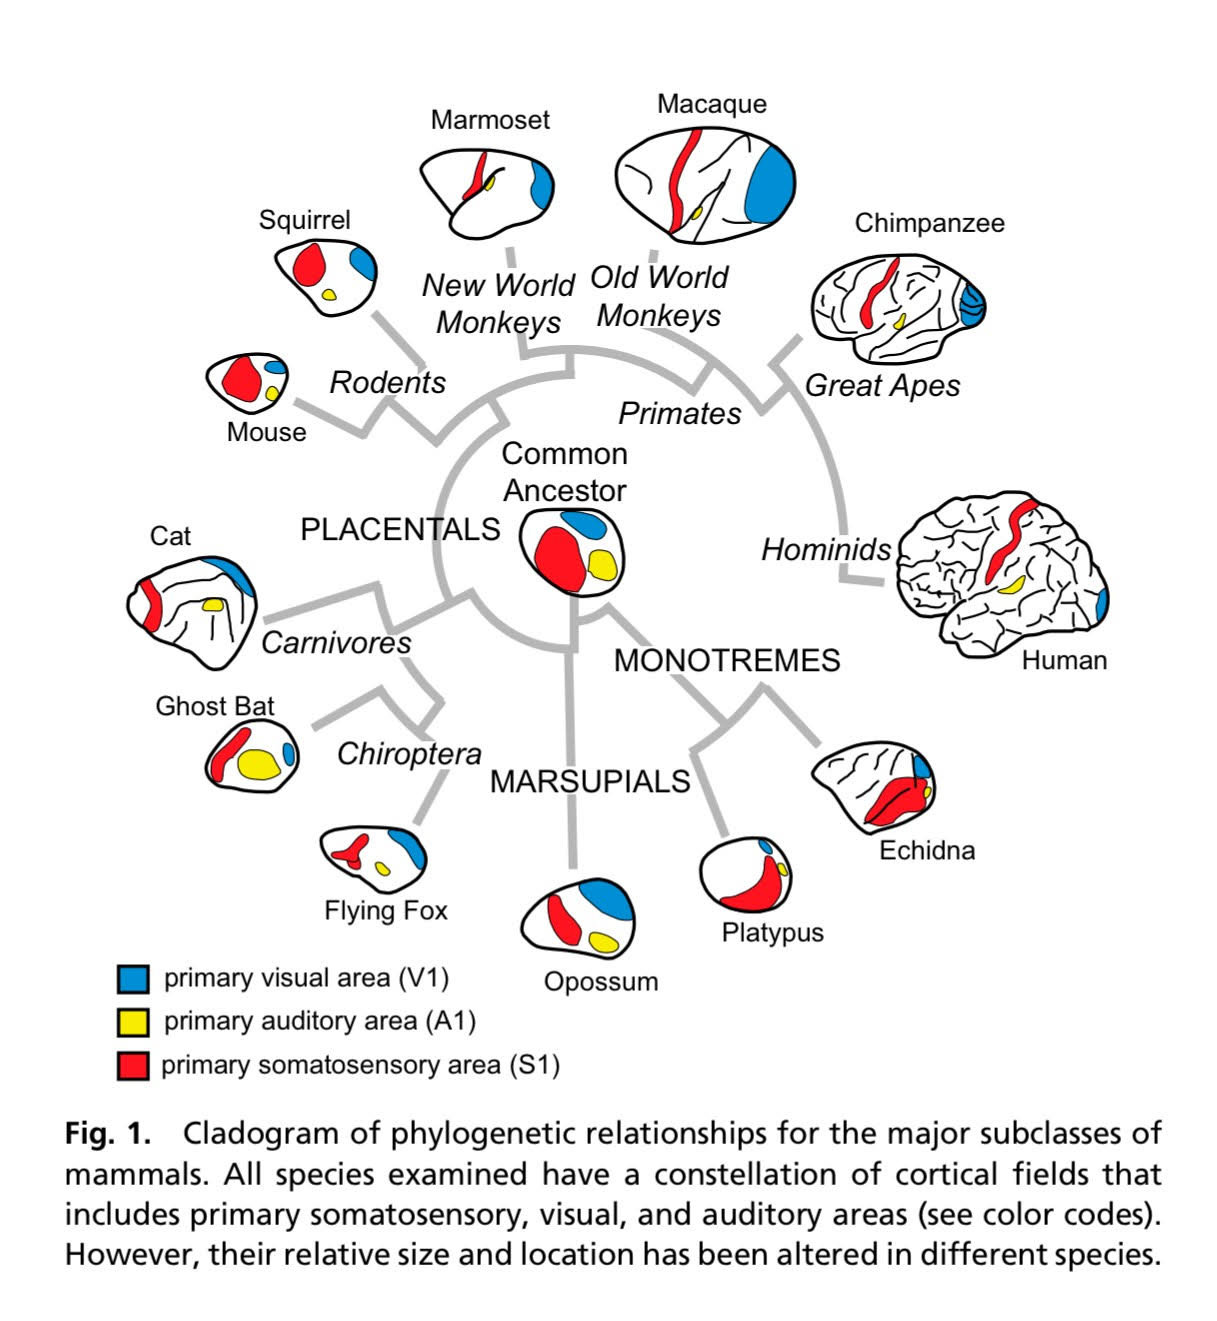
\includegraphics[width=\linewidth]{mammals.jpg}
  \caption{\emph{Varying cortical areas in mammals}. Source: \citealp{Krubitzer2012}}
  \label{fig:mammals}
\end{figure}

The development of connections from the thalamus to the cortex involves phenomena such as neurogenesis, cell migration, neuronal differentiation and axon guidance. Here we focus on how axons are guided to distinct areas of cortex. Models such as \cite{Karbowski2004} explain how gradients of morphogens, which guide the axons into distinct areas, can emerge through their interactions with each other. Each gene produces the responsible proteins for axon guidance while at the same time activating or deactivating some of the other genes. These networks of interactions are called Gene Regulatory Networks (GRNs) and are extremely common biological systems.\par

It is known that the gradients of five morphogens influence axon growth in the developing cortex. Fgf8, Pax6 and Sp8 have higher anterior concentrations than posterior, where as Emx2 and Coup-tfi have opposite gradients, increasing towards the posterior (see figure \ref{fig:gradients}).\par

\begin{figure}[h]
  \centering
  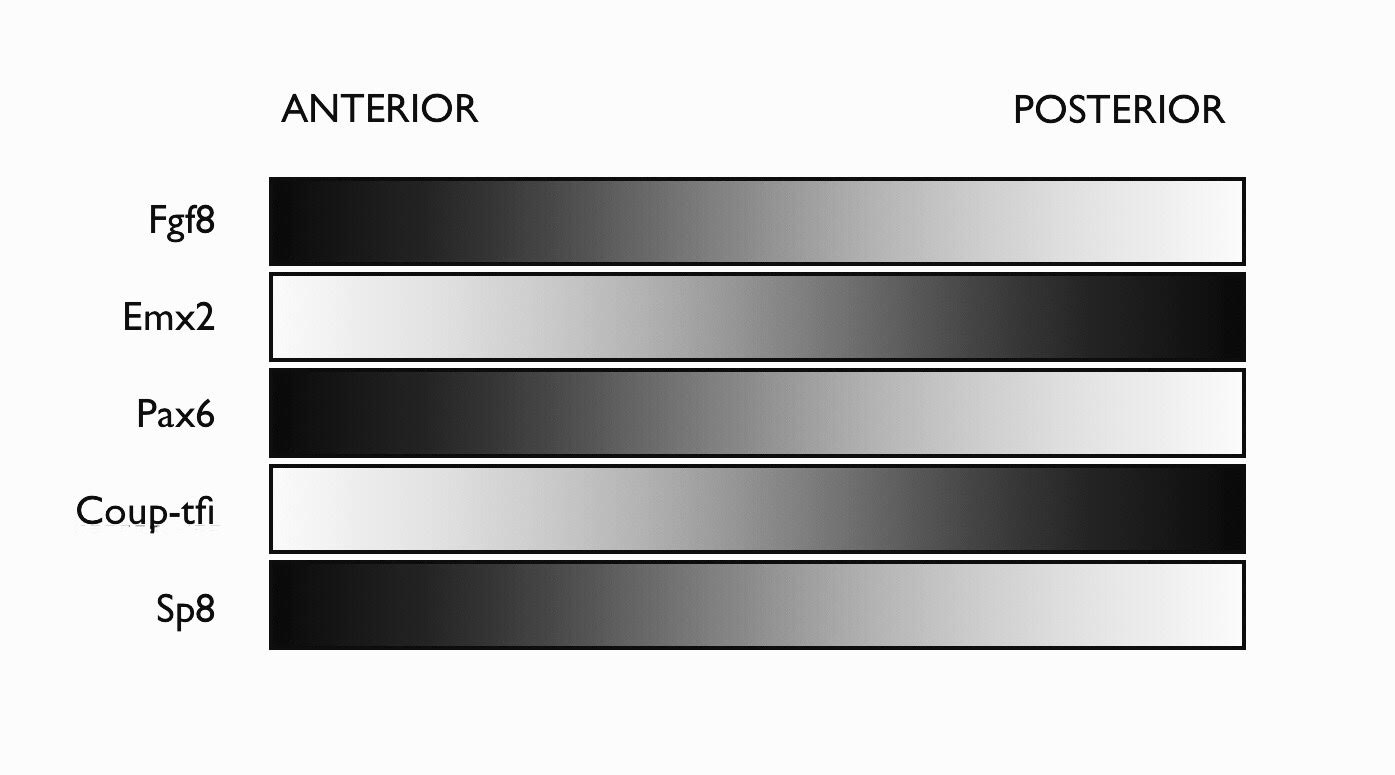
\includegraphics[width=\linewidth]{gradients.jpg}
  \caption{\emph{Morphogen gradients}. The expression levels of five proteins where a darker shade represents a higher concentration. These gradients provide a co-ordinate system which guides axons from the thalamus to the cortex, creating boundaried areas.}
  \label{fig:gradients}
\end{figure}

These gradients are established by each gene being regulated by the others, in a GRN. So for example, the Sp8 protein will cause the transcription of the Fgf8 gene to increase, the resulting Fgf8 protein may then inhibit the transcription of the Sp8 gene. A more realistic example of a full network is given in figure \ref{fig:network}.\par


\afterpage{
\begin{figure}
\begin{center}
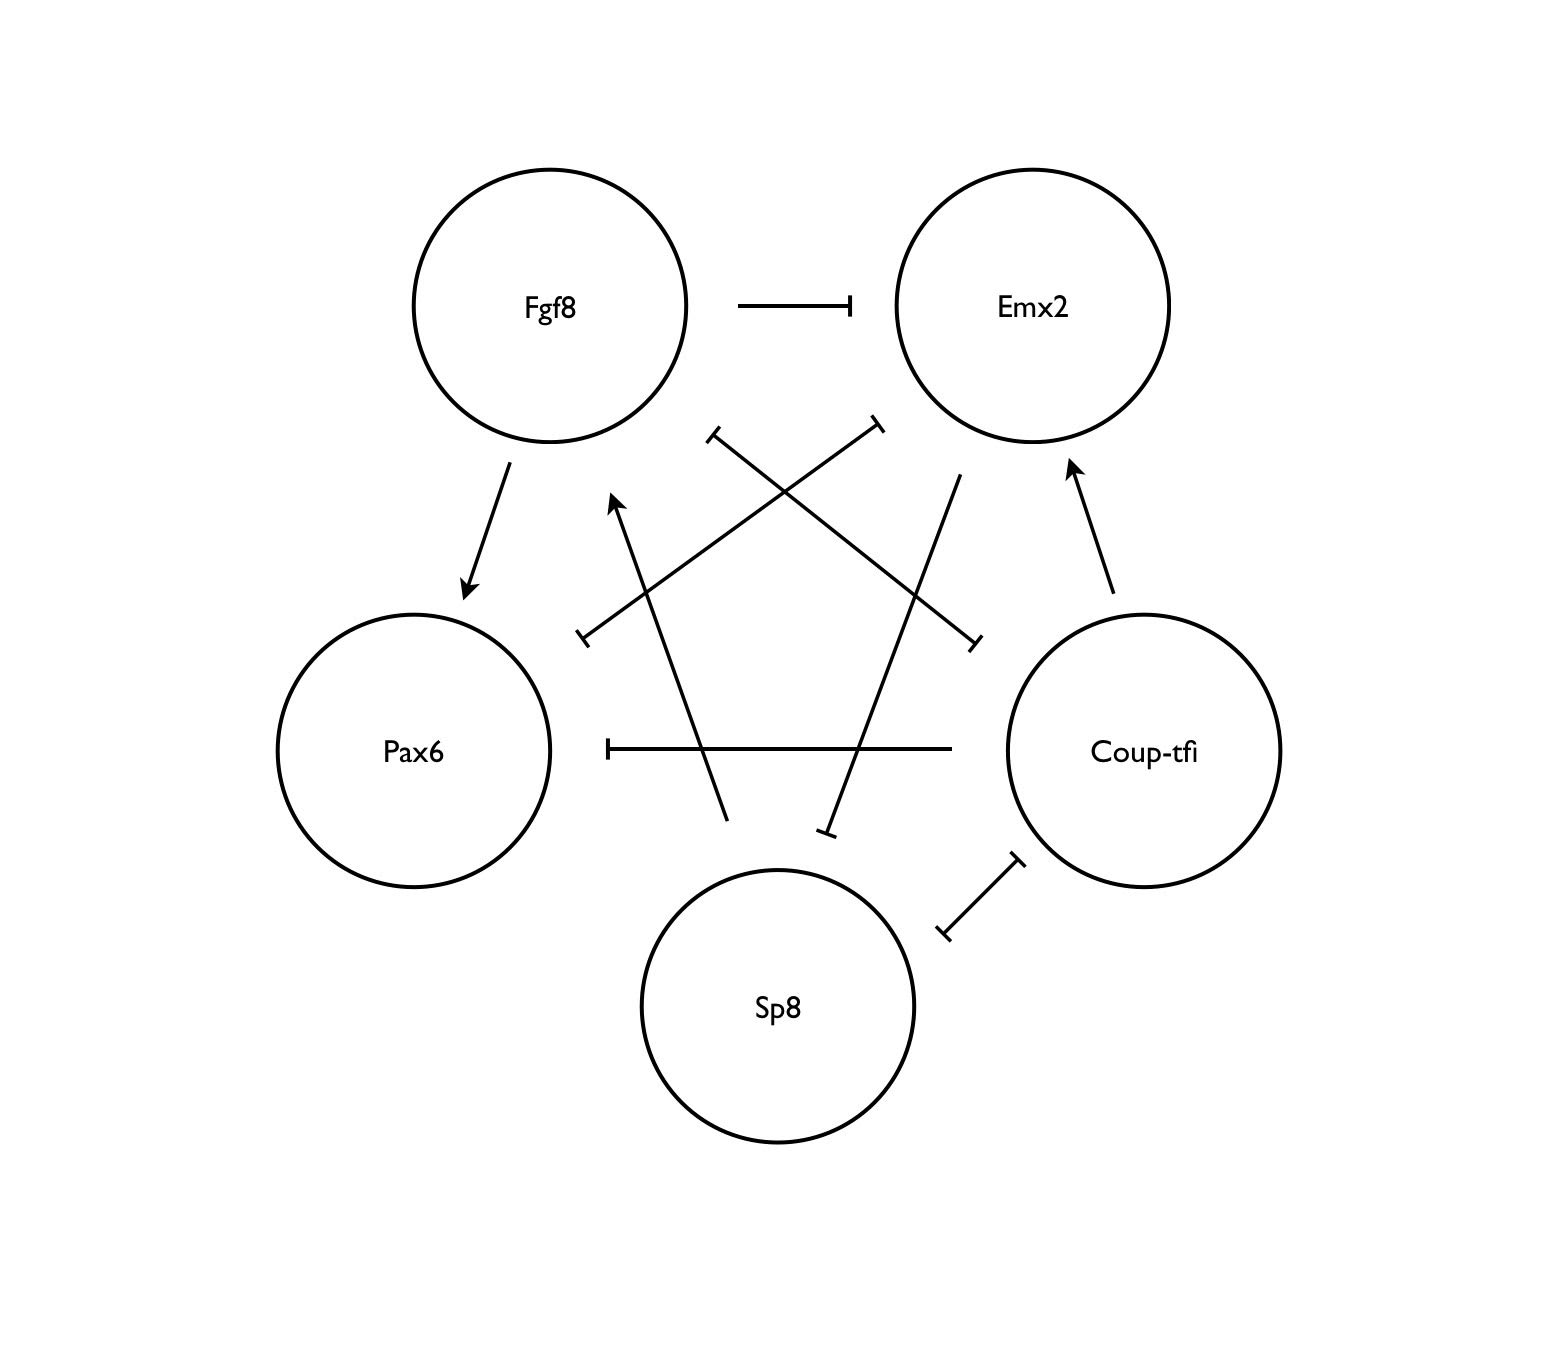
\includegraphics[width=1.0\textwidth,clip=true,trim=0cm 0cm 0cm 0cm]{network.jpg}
\caption{\emph{A feasible network}. The figure represents the activating ($\rightarrow$) or inactivating ($\dashv$) interactions between five genes. This particular network is only demonstrative, the actual interactions responsible for cortical arealisation are unknown.}
\label{fig:network}
\end{center}
\end{figure}
\clearpage}

This may seem like an overly complicated way of setting up the necessary gradients, wouldn't a simpler way be to just emit the desired proteins from each pole and let them diffuse across? This system may provide a way for all mammals to have a basic set of cortical areas while making it easy to modify for each species' niche. Or perhaps it provides a way for the evolutionary process to be influenced by development, which could speed up the exploration of the phenotypic space. This is the hypothesis which we will explore later.\par

Gene regulatory networks can be modelled in a detailed way through reaction-diffusion equations, which describe the concentrations of the morphogens as a continuous function in space. Simpler models, such as Boolean Networks, can be useful by limiting the level of detail to whether genes are active or inactive in a particular domain, rather than allowing them a range of activity.\par

\subsection{Boolean Networks}

Boolean Networks were intially used to model gene interactions by \cite{Kauffman1969}. He studied networks where the interactions were randomised and found that even random networks could predict features of real cells. He was interested in the interaction between self-organisation and natural selection, he worked with Per Bak who later developed a successful evolutionary model \citep{Bak1993}. Since then many different types of boolean nets have been formulated, each with advantages for particular situations \citep{Bornholdt2008}. We will use cortical arealisation to test our formulation against other established results, before using the model in an evolutionary context.\par

Firstly, to explain how boolean networks function let's take a simple example of a random boolean network, like Kauffman's original. Let's say the network has three nodes, or genes, X, Y and Z. Each gene can either be active, `1', or inactive `0', so at a particular timestep the state of the system may be `XYZ' = `110'. With N genes there are a total $2^N$ possible states, in this case 8. Which state the network is in at one time is what decides the activity of the nodes at the next timestep. The table below gives one example of how the activity of node X could be decided by the 8 possible states.\par
\vspace{2em}
\begin{center}
  \begin{tabular}{| c | c |} 
    \hline
    Input (XYZ) & Output (X) \\ 
    \hline  
    000 & 1 \\
    001 & 0 \\
    010 & 0 \\
    011 & 0 \\
    100 & 1 \\
    101 & 0 \\
    110 & 1 \\
    111 & 1 \\
    \hline
  \end{tabular}
\end{center}
\vspace{2em}
It is the output column in the truth table that is randomised, for node X alone there are $2^8$ possible logical functions. For all three nodes there are a total $2^{24}$ possible truth tables, each of which represents a different network, below is one example.\par
\vspace{2em}
\begin{center}
  \begin{tabular}{| c | c |} 
    \hline
    Input (XYZ) & Output (XYZ) \\ 
    \hline  
    000 & 101 \\
    001 & 011 \\
    010 & 001 \\
    011 & 010 \\
    100 & 111 \\
    101 & 001 \\
    110 & 100 \\
    111 & 111 \\
    \hline
  \end{tabular}
\end{center}
\vspace{2em}
Each network's truth table fully determines the dynamics of state transitions, and each network will give different dynamics. The full dynamics can be visualised in `state space', for the particular example above this is shown in figure \ref{fig:statespace}. With this type of boolean network every state will develop towards either a `point attractor' or `limit cycle', but the size and location of these attractors differs for every network.\par 

\afterpage{
\begin{figure}
\begin{center}
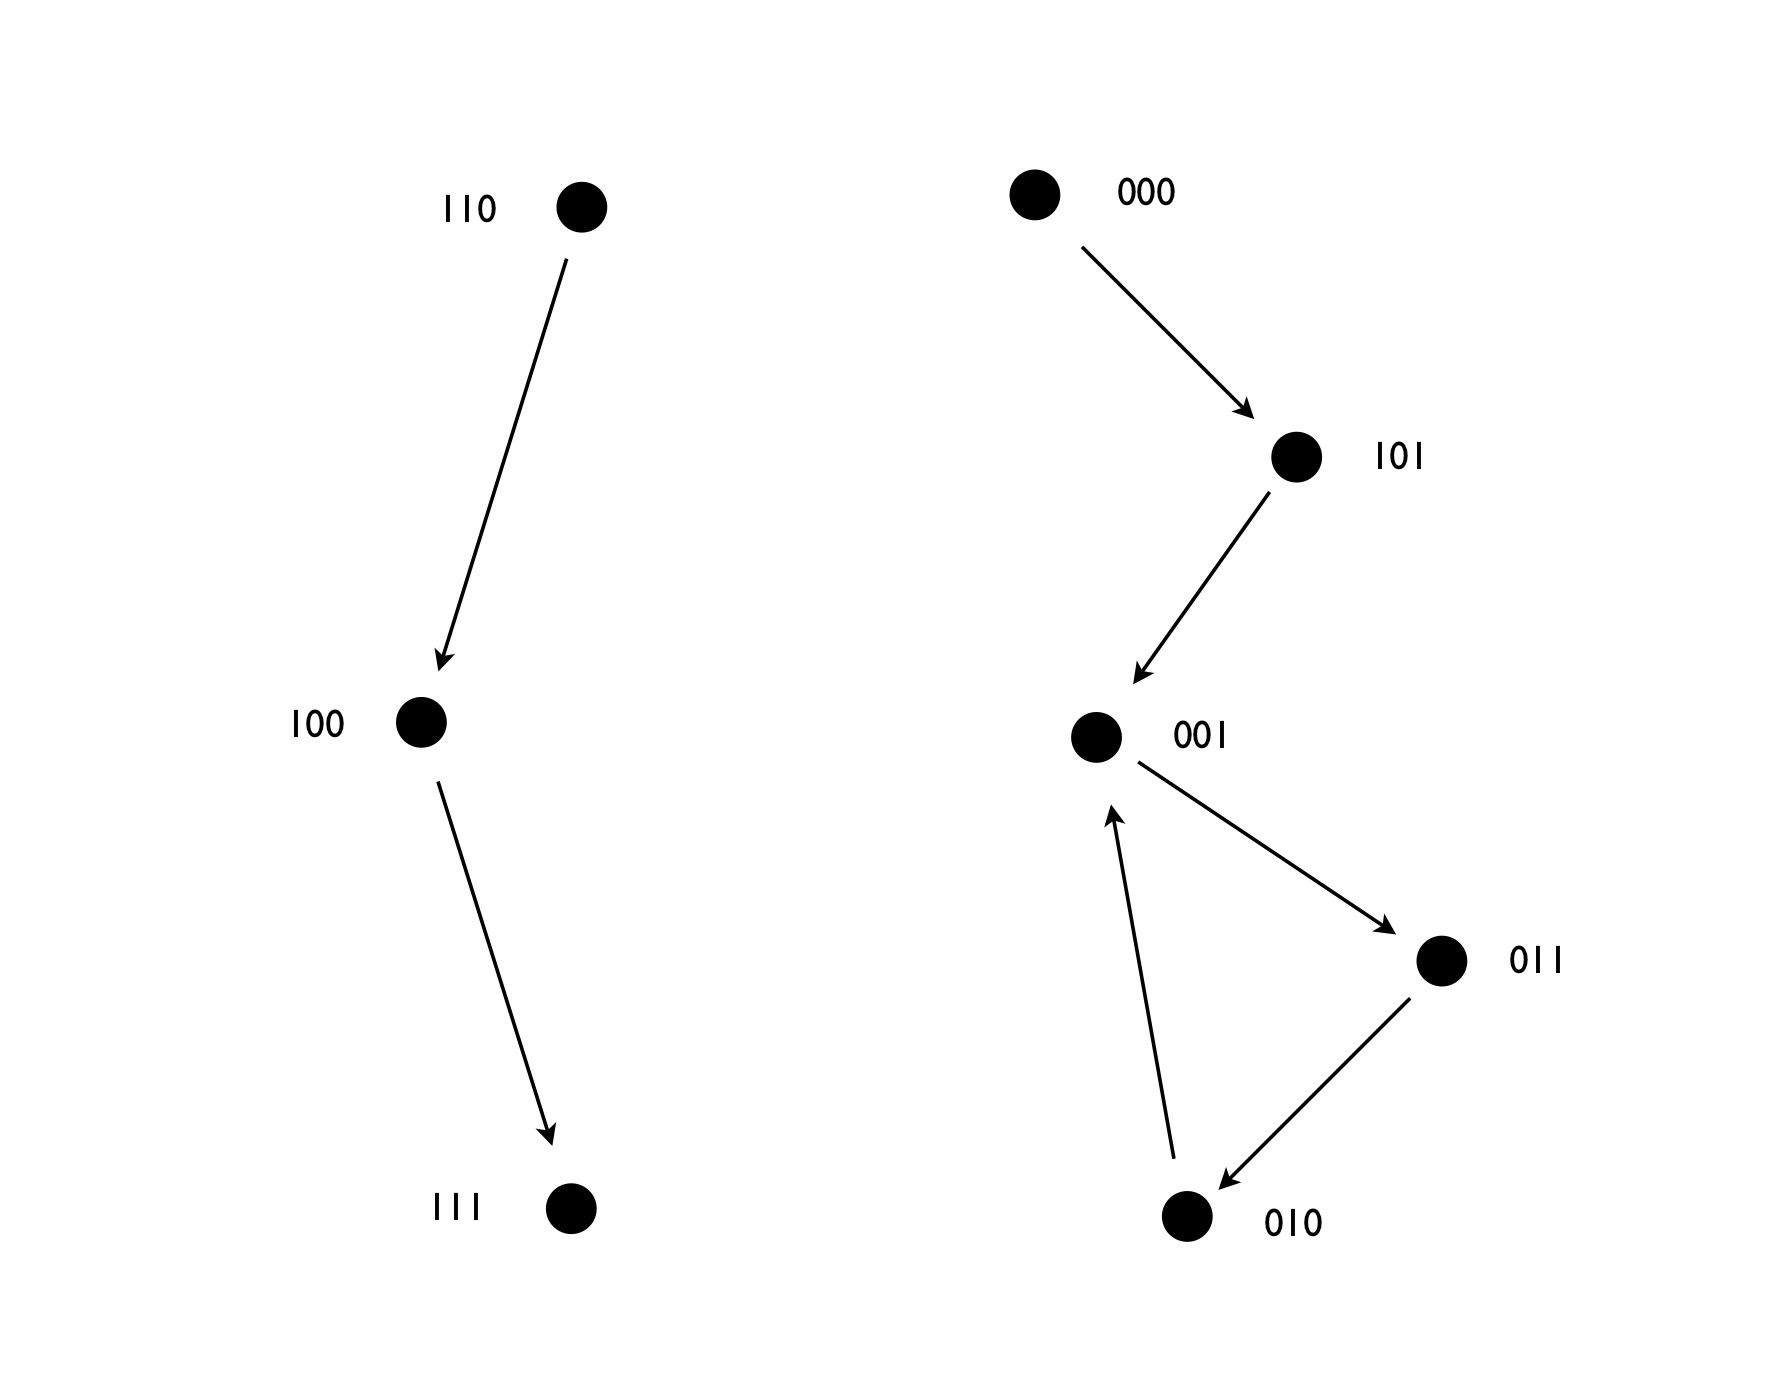
\includegraphics[width=1.0\textwidth,clip=true,trim=0cm 0cm 0cm 0cm]{statespace.jpg}
  \caption{\emph{The dynamics of a random three-node boolean network}. Each black dot represents a state which is labelled by the activation levels of the network's three nodes. Each state transitions deterministically, creating two basins of attraction, on the left is a `point attractor', on the right is a `limit cycle'.}
  \label{fig:statespace}
\end{center}
\end{figure}
\clearpage}


To compare different networks we can reduce the information from the state space diagram down to one dimension, just the values of the attractors along the x-axis, and use the y-axis to stack each network on top of each other. In figure \ref{fig:close} we use this idea to compare the network above with three networks which are only one bit different.

\afterpage{
\begin{figure}
\begin{center}
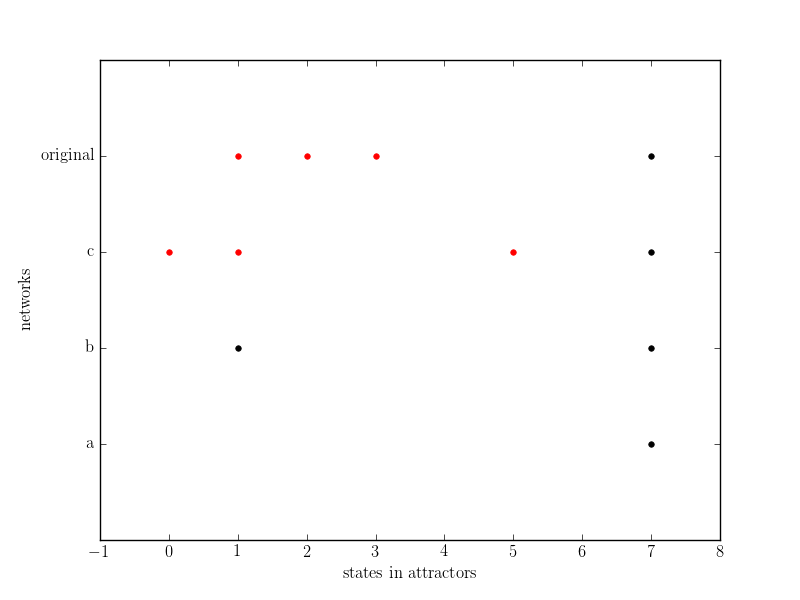
\includegraphics[width=1.0\textwidth,clip=true,trim=0cm 0cm 0cm 0cm]{close.png}
  \caption{\emph{Attractor diagrams for 4 nearby networks}. The original network is the one visualised in figure \ref{fig:statespace}, where the state 001 transitions to 011, in networks a,b and c the state 001 transitions to 111, 001, and 010 respectively. So each of these networks have only one bit different from the original in their truth tables. The black markers shows states that are point attractors, the red markers show states that are in limit cycles.}
  \label{fig:close}
\end{center}
\end{figure}
\clearpage}

Our results will be compared to the model of \cite{Giacomantonio2010}, (henceforth referred to as `the original model' or `the Goodhill model'). They simplified the morphogen gradients by splitting the cortex into two domains, with each domain having concentrations represented by binary states. So the  empirically observed gradients would have a state such as `10101' in the anterior and `01010' in the posterior, where each bit in these strings, from left to right, corresponds to gene activation of Fgf8, Emx2, Pax6, Coup-tfi and Sp8.\par

Similarly, the initial states of the system have been observed to be `10000' (anterior) and `00000' (posterior), where the 1 is the presence of Fgf8. Each boolean network provides a different path from these initial states, some of which will end up in the desired states mentioned above. There are $2^{24}$ possible networks, given the constraints that the authors chose, representing many potential interactions between the 5 genes. By trialing the evolution of states in every possible network they found a small subset, about 0.1\%, which would lead to the desired final states.\par

We aim to recreate the Goodhill model, but with deterministic Boolean Networks. By doing so we will be able to visualise the entire state dynamics for a given network, rather than a single trajectory as Goodhill did, this will give an indication of how robust the system is to slight changes in the initial conditions. We will find whether the most successful networks in the original model match ours, and whether the frequency of particular interactions, for example Fgf8 inhibiting Emx2, is comparable.\par

\subsection{Fitness Landscapes}
We will then use our deterministic model to investigate how development might aid or constrain evolution. To do this we make an analogy between the network and the genotype, and between the resultant dynamics and the development of the phenotype. Each network has a `genome' which is the string of bits encoding its truth table, each giving a different outcome in state space, with attractors of different sizes and locations.\par

The previous models used a very constrained definition of fitness, if the states developed exactly as desired then the network has fitness 1, but any other network has 0 fitness. With 5 genes, and all possible logical operators, there are a possible $2^{160}$ networks for evolution to search through. This is a very large space to find networks of peak fitness, if other nearby networks give the organism some middling level of fitness, then the fitness ‘spikes’ would be broadened, making the peaks easier to find.\par

We used random boolean networks to explore the fitness landscape, finding relevant statistics to compare different fitness functions. The boolean network ‘genomes’ can be represented as an 80 bit binary string, which means the fitness landscapes we are exploring are 80 dimensional and not easy to visualise. Still, some basic structure of the landscape can be understood, like how rough or smooth it is, by looking at how the evolutionary algorithm explores the space.\par

\newpage{}
\section{Models}
The majority of assumptions in our model are the same as in the original model. These are described in detail here. Both models describe the activation levels of five genes, and the presence of their respective proteins, each of these ten variables can take the value `1' or `0'. Many possible interactions are constrained, genes do not interact directly with genes, nor proteins with proteins, rather the presence of a protein could activate or inactivate any of the genes, and each gene can cause the presence of its respective protein.\par

Both models deal with time in discrete steps, with each value being determined only by the values in the single previous timestep. This corresponds to a biological assumption that gene and protein levels must be permanently regulated, i.e mRNA and protein is synthesised or degrades in one time step.\par

The interactions are also constrained in that they are limited to representing only AND or NOT  logical functions. This is an enormous constraint, if each of 5 genes is regulated by 5 proteins and there are 3 possible interactions (AND, NOT and no interaction), then there are $3^{25}$ possible Boolean Networks. If all logical functions were permissible then that number would be $2^{160}$, so there are roughly a factor of $10^{36}$ more than are being considered. This may not be a fair assumption as there is evidence that in real gene regulatory networks there exists complex functions of AND, NOT and OR operators \citep{Alon2007}.\par

Two further constraints bring the number of possible networks down again. As we are looking at five genes with opposite gradients, we can assume that excitatory interactions between those of opposite gradients will not exist in successful networks, similarly, inhibitory interactions will not exist between genes with the same gradients. For example, Fgf8 cannot indirectly activate Emx2, or inhibit Pax6. The final constraint is that the Sp8 protein will always activate the Fgf8 gene, as this is well established empirically. This leads to a total of $2^{24}$ possible networks, whose interactions are selected from the table in figure \ref{fig:table1}.\par

\afterpage{
\begin{figure}
\begin{center}
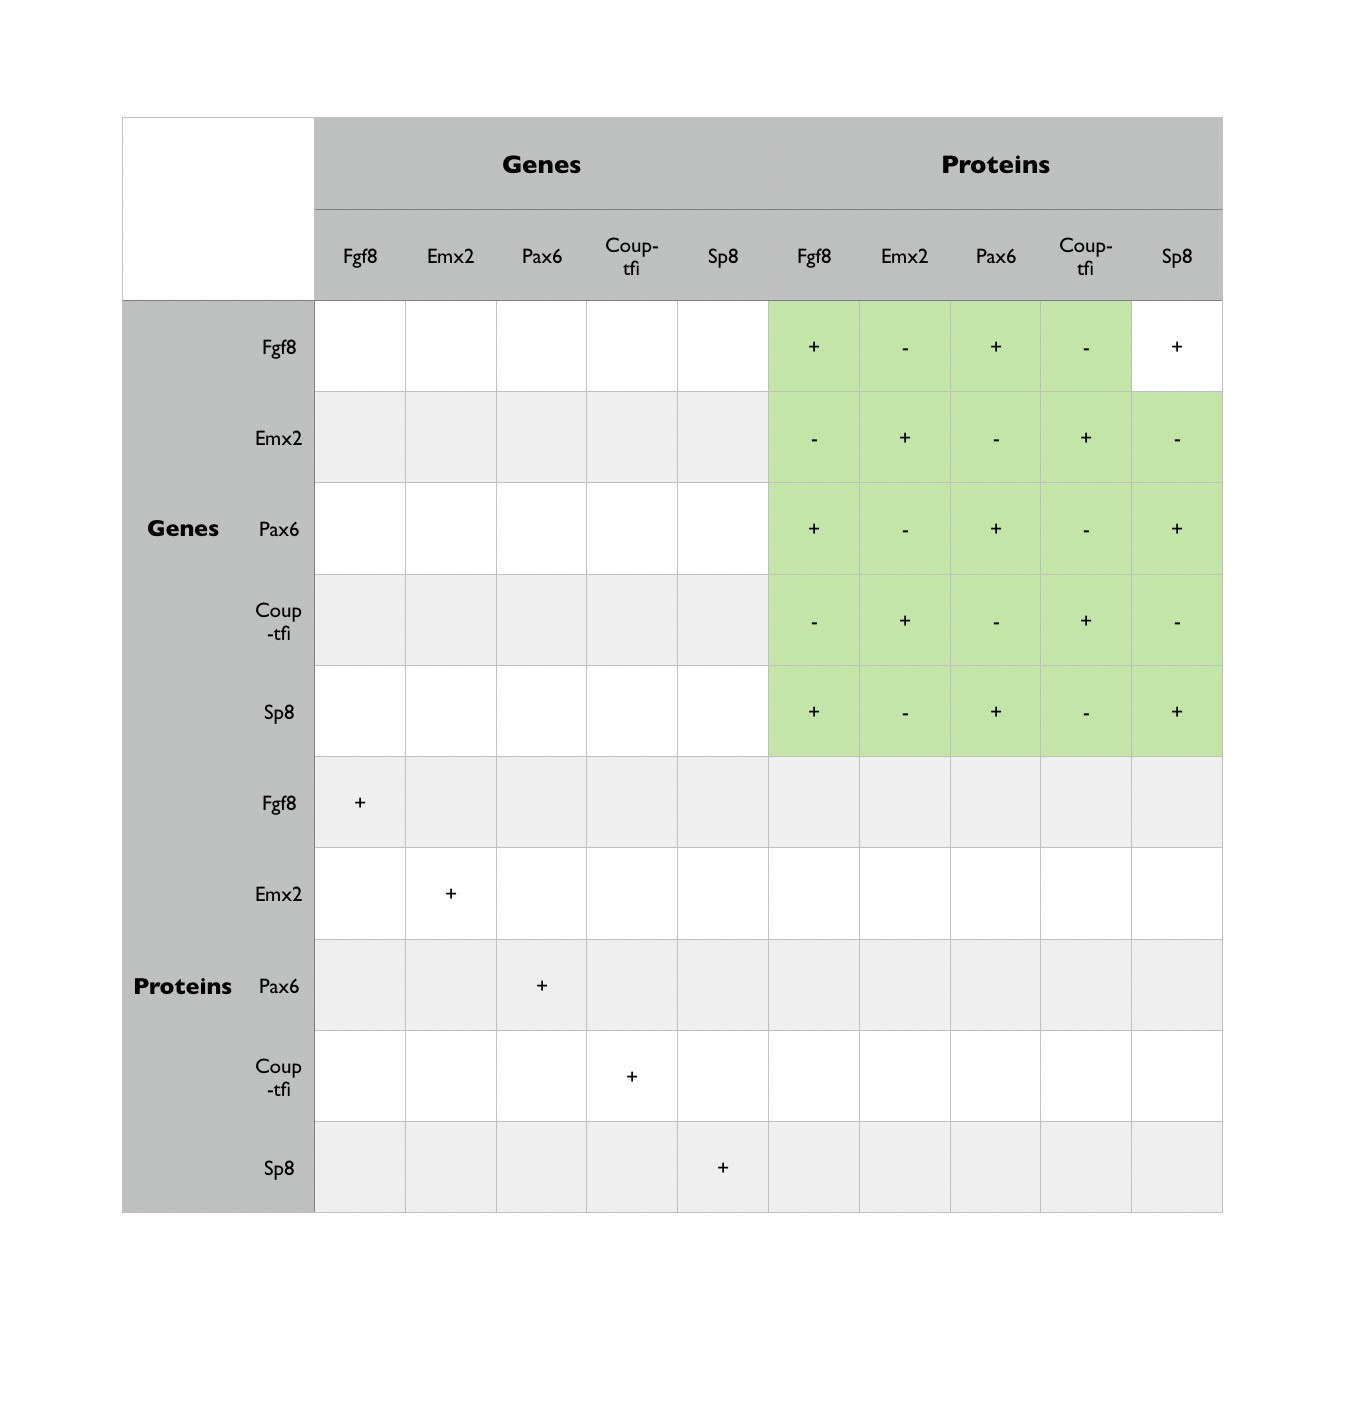
\includegraphics[width=1.0\textwidth,clip=true,trim=0cm 0cm 0cm 0cm]{table1.jpg}
  \caption{\emph{Possible interactions for our networks}. The space of all potential interactions is massively constrained to the smaller set in this figure. The interactions shaded green are the ones to be trialed in all possible combinations, where as the non-shaded interactions are fixed for all networks. Each `+' interaction is included with an AND operator, each `-' involves a NOT interaction.}
  \label{fig:table1}
\end{center}
\end{figure}
\clearpage}


\subsection{Synchronous or Asynchronous?}
The only real difference between our model and the original is that they chose to transition between states asynchronously and stochastically, where as we have chosen to update the states synchronously and deterministically. In both implementations the deterministic state table first has to be computed, this is the full list of $2^{10}$ states and their consequent state in the next time step. In our model this is where we stop and draw the resultant attractors for that network. In the Goodhill model they add an extra step which is to assume that changes to the state only happen one at a time, and with equal probability. For example, in our model the state `00010' could transition to `11010', in the original model it would have probability of 0.5 to be `10010' or `01010', as there are 2 changes in the state.\par

The probability is calculated for each state to transition to every other, creating a `transition matrix'. Using this matrix the probability of ending up in a steady state from any transient state can be calculated analytically or numerically. Giacomantonio and Goodhill chose to computationally progress through states until there was a 99.99\% chance of being in the steady state.\par

The merits of synchronous or asynchoronous models are a controversial matter which will be explored in more detail in the Discussion section. Suffice it to say here that the original model chose asynchrony for two main reasons, they deem it to be more biologically feasible and it removes the complication of limit-cycles. However, we have chosen a synchronous model because we question the biological feasibility of reducing transitions probabilistically, and it is the limit-cycles and other state space dynamics that interest us. \par

Cellular processes such as transcription, translation and degradation have different timescales, so it is reasonable to assume that if two genes become active their respective proteins will not be available at the same time. So while asynchrony does seem more biologically feasible, we feel that the original model does not reflect that in its implementation. For example, consider a single protein that activates two genes, it is likely that the genes become active over differing time spans, first one and then the other. But it seems unreasonable that 50\% of the time one gene would become active, or else the other gene does, always one of them and never both.\par

Therefore, our model is synchronous and deterministic, this gives us full state space dynamics for each network, allowing us to make an analogy with the development of an organism.\par


\subsection{Points of comparison}
The key aim of the original model is to reduce the large set of $2^{24}$ possible networks down to a much smaller sub-set of `good' networks. They found that 0.1\% of all networks produced the desired expression patterns. Therefore we will also run the model for every possible network and count the number of successful networks. Success is defined as the anterior state `1000010000' (Fgf8 present), leading to the point attractor `1010110101' and the posterior state `0000000000' leading to the point attractor `0101001010'.\par

In their paper, Giacomantonio and Goodhill gave examples of two networks which they said performed the best. We are interested to see if these networks are also successful in our model. However, we can also look at the full state-space for these networks and judge how robust their success is (or is not).\par

We would like to find the frequency of particular interactions within successful networks and compare these with the original model. Goodhill found that successful networks never had autoregulation and that inhibitory interactions were much more common, will we find the same?\par

Finally, it will be interesting to visualise how the attractor space varies for networks that are local to each other. Is there any smoothness to the function which maps networks to the state space?\par

\subsection{Models for evolutionary dynamics}
The model we are using to investigate the structure of the fitness landscape is also deterministic, but simplified and more general. We returned to the original conception from \cite{Kauffman1969} of a random boolean network, with 5 nodes that each connected to the 4 other nodes. There are $2^{N2^{N-1}} = 2^{80}$ possible truth tables for such a situation, meaning a`genome' of 80 bits can comprehensively encode all possible networks.

It would be computationally impossible to find the fitness of all $2^{80}$ networks and plot the resultant fitness landscape. However, it is sufficient to take a random sample. An undirected random sampling can be compared to a directed evolutionary search through the space. This gives an indication of whether the space is structured in a way which allows evolution to find optimal networks more quickly than a random search would.\par

The evolutionary algorithm takes a ‘genome’, which is a string of 80 bits representing one possible network, measures its ‘fitness’, it then flips each bit with a probability, p, and measures the fitness of the new resulting genome. The least fit genome is discarded and the process repeats. The number of generations until the algorithm reaches the maximum fitness is counted for many trials of this process, giving a frequency distribution. This frequency distribution, for various values of p, is the key statistic that gives us information about the structure of the landscape.\par

To understand how this statistic varies for different landscapes we tested two null models, one was perfectly rough (random fitness), the other perfectly smooth. If the network space was one dimensional then this smooth fitness function would look like a straight line from 0 fitness to 1. This smoothness was achieved by correlating the fitness to the number of ‘1’s in the genome, so for any network a single mutation will take the fitness slightly up or downhill.\par

We then created a new fitness function, the aim of which was to have the same maximal and minimal values as the original Goodhill model, but to give some networks medium levels of fitness. The function still has optimal fitness for the states `10000' and `00000' leading to `10101' and `01010' respectively. But now if the final state is one bit different to the desired state, fitness will be reduced by 0.1. We chose this function to allow a spectrum of values depending on the network's development in state space, to see the effect on the evolutionary statistics.\par

The fitness, f is defined by;
\begin{equation}
f = 1 - 0.1 \times d
\end{equation}
where d is the total Hamming distance of both final states from the desired states. For example if the state `10000' developed to a point attractor `10111' rather than `10101', but the initial state `00000' developed as desired, the fitness would be reduced to 0.9. If the network develops into a limit cycle rather than a point attractor then the fitness is deemed to be zero.\par




\newpage{}
\section{Results - Evaluation of deterministic model}


\subsection{Proportion of networks that are successful is 0.01\%}
The code in `proportion.py' systematically goes through each of the 16,777,216 ($2^{24}$) possible networks, if the network passes the criteria of success it is added to a list. The list of all successful networks can be found in `successes.txt'. In total there were 1,710 successful networks, so a proportion of 0.0001. This is on the same order as the proportion of networks deemed to be good by the original model, 0.00035 (5,849 networks). This is lower than their other quoted value of 0.1\% because they also rejected networks that contained features such as auto-induction or isolated repressive loops, which generally failed to produce the desired gradients. Whichever value from their paper is chosen for comparison, the proportion is reasonably close, and importantly supports the goal of vastly reducing the space of candidate networks. 

\subsection{The best networks from the original model were not successful}
Although the proportion of successful networks is comparable it is possible that our model gives a very different subset to the original. Unfortunately, we do not have access to a full list of successful networks from the original model, the authors only publish the `best' two networks. They refer to them as the `best performing networks' because their model is probabilitic and these networks have the highest probabilities of reaching the desired steady states. In our deterministic model all of our networks have equal status of being entirely successful or not at all.\par

We ran our model for the best two networks from the original model and found that neither of them was successful. By visualising the state space for each network (figures \ref{fig:best-a} and \ref{fig:best-b}) we can see that they were close to being successful and why they failed, for comparison there is also the state space for a successful network and a random one (figures \ref{fig:success} and \ref{fig:random}).\par


\afterpage{
\begin{figure}
\centering
\subfloat[]{
    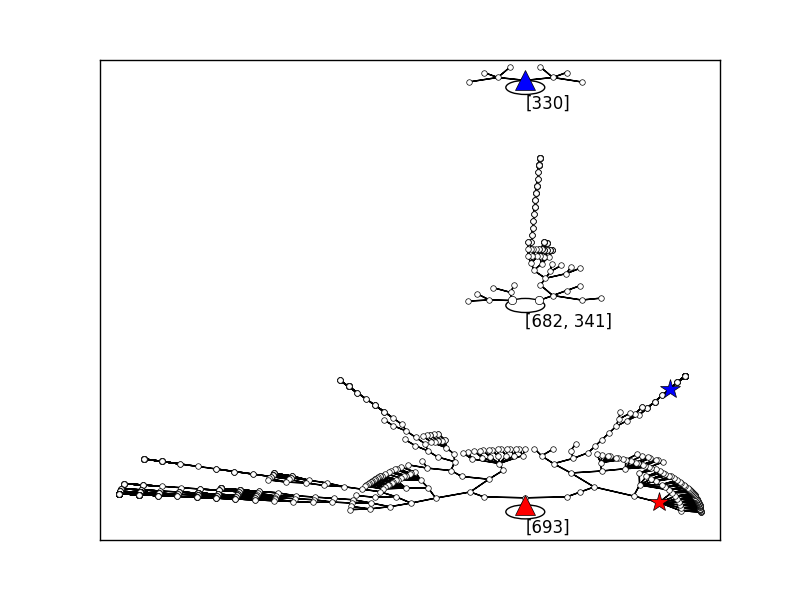
\includegraphics[width=0.8\linewidth,clip=true,trim=0cm 0cm 0cm 0cm]{best-a.png}
    \label{fig:best-a}}

\subfloat[]{
    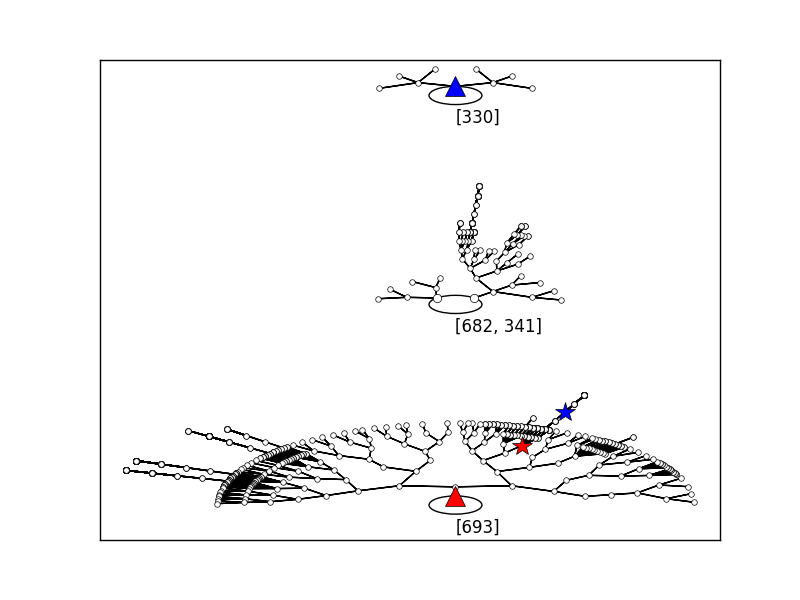
\includegraphics[width=0.8\linewidth,clip=true,trim=0cm 0cm 0cm 0cm]{best-b.png}
    \label{fig:best-b}}
    \phantomcaption
\end{figure}
\clearpage}
\afterpage{  
\begin{figure}\ContinuedFloat
\centering
\subfloat[]{
    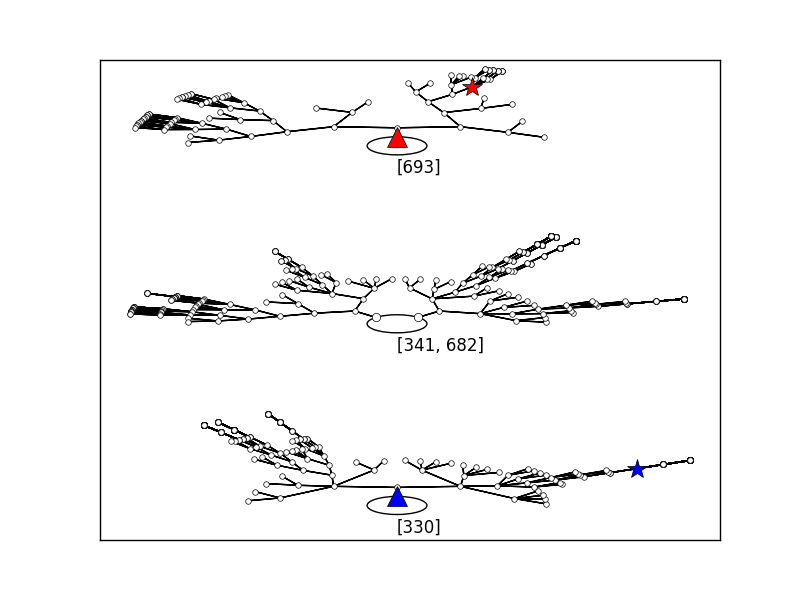
\includegraphics[width=0.7\linewidth,clip=true,trim=0cm 0cm 0cm 0cm]{success.png}
    \label{fig:success}}

\subfloat[]{
    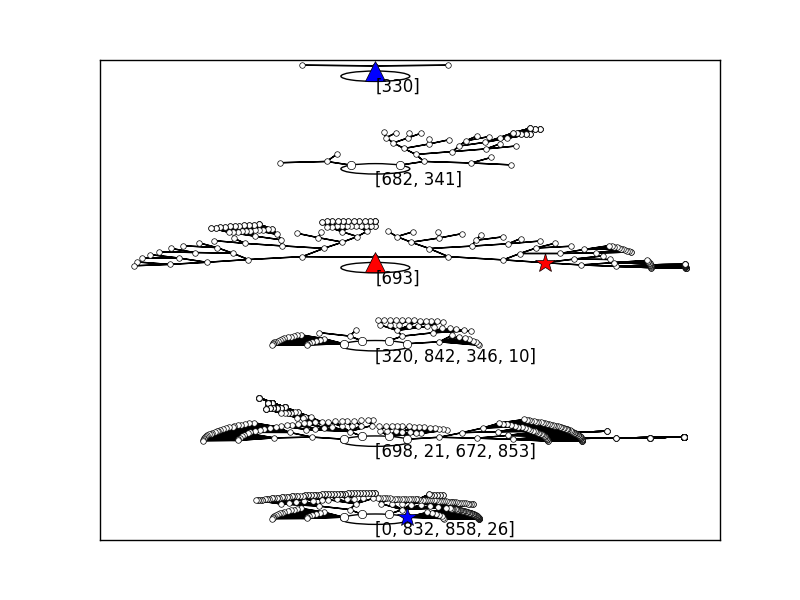
\includegraphics[width=0.7\linewidth,clip=true,trim=0cm 0cm 0cm 0cm]{random.png}
    \label{fig:random}}
  \caption{\emph{State spaces of four networks from our model}. Each figure depicts the dynamics of a different network, with each node representing a particular state which leads deterministically to another state, and eventually to a limit-cycle or point attractor. The states in the limit-cycle are labelled with the decimal conversion of their binary state. The triangles mark the location of the desired final state red for anterior (693), blue for posterior (330), the stars mark the initial states, with the same colouring. \textbf{(a)} and \textbf{(b)} show the best networks from the Goodhill model, they both have the correct attractors but the posterior initial state will not develop correctly. \textbf{(c)} shows a successful network. \textbf{(d)} shows a random unsuccessful network for comparison. The code to reproduce these figures can be found in `best2.py'.}

\end{figure}
\clearpage}


\subsection{The frequencies of particular interactions are almost identical between models}
Although the Goodhill paper didn't provide a list of all successful networks it did state the frequency of particular interactions throughout all `good' networks. Using the code in `interactions.py', we found the frequency of each interaction and created figures \ref{fig:freq-correlation} and \ref{fig:freq-dist} which show how our model gives very similar results. Figure \ref{fig:freq-table} shows the frequency of each interaction for successful networks in both our model and the original.\par


\afterpage{
\begin{figure}
  \centering
\subfloat[]{
    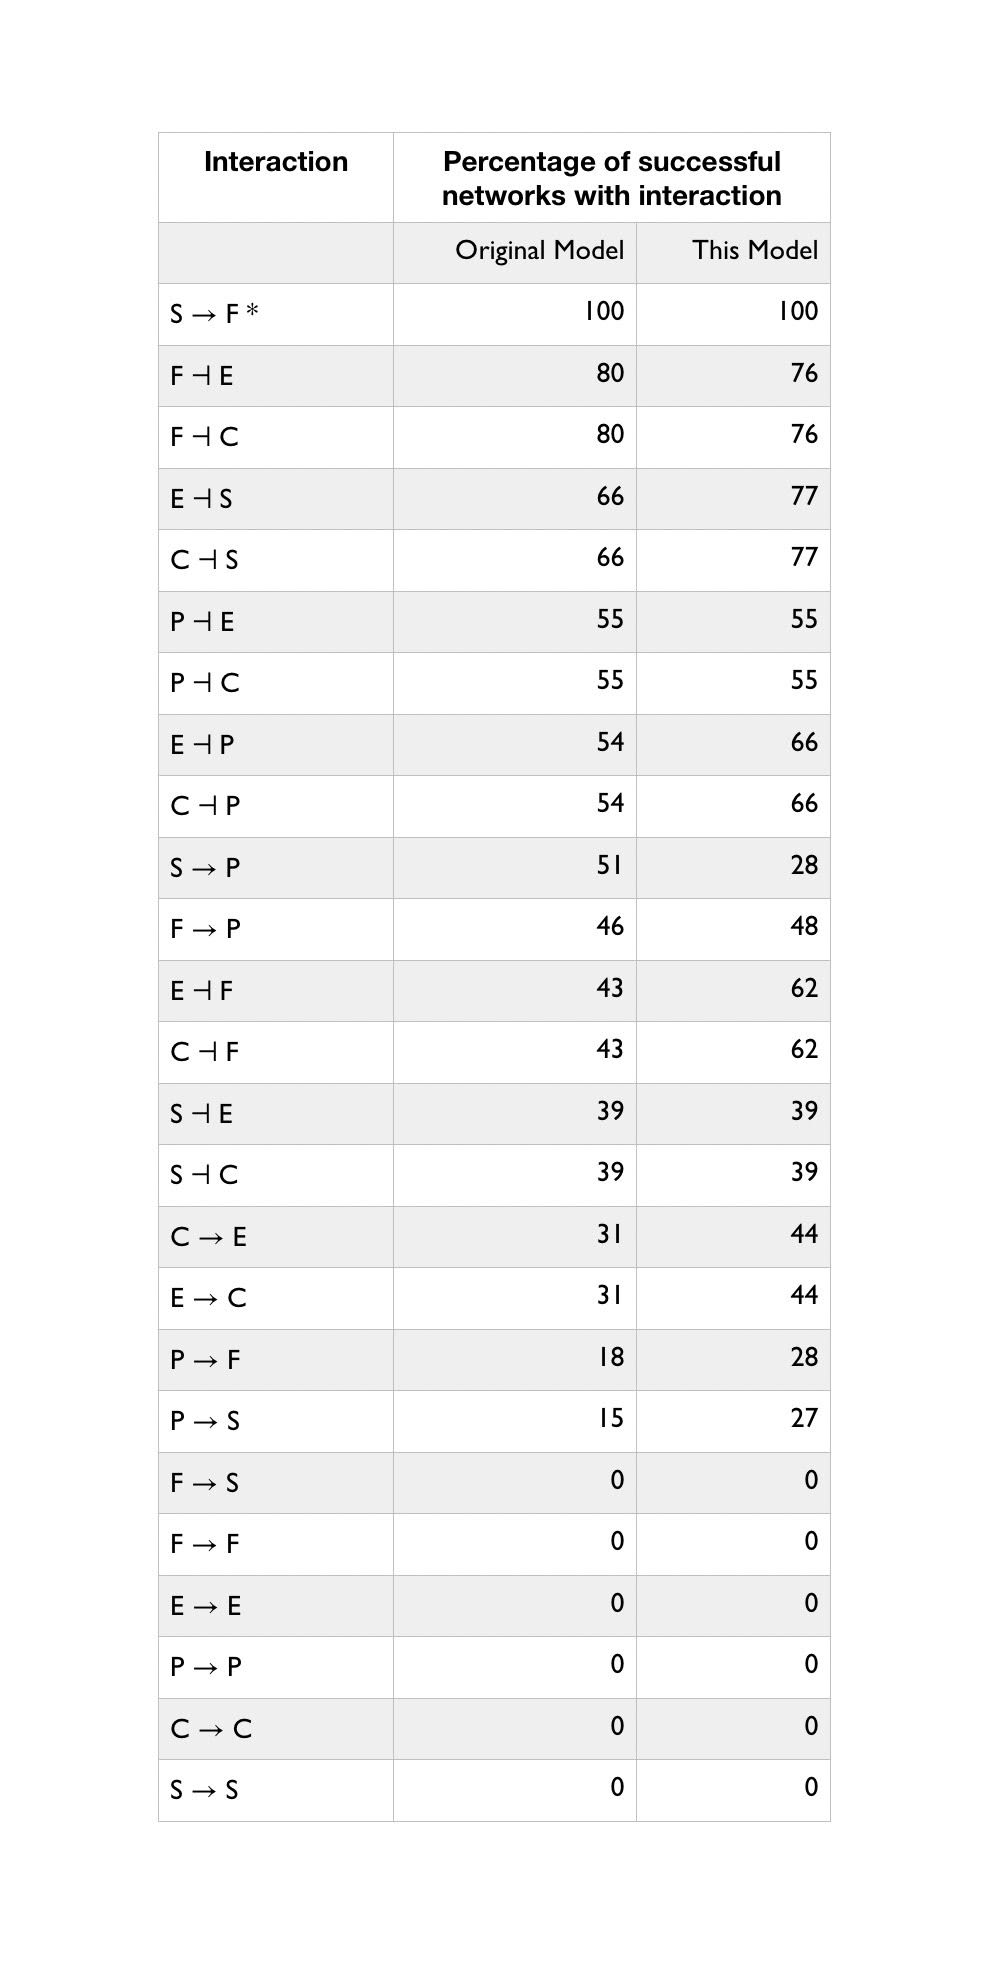
\includegraphics[width=0.6\textwidth,clip=true,trim=0cm 0cm 0cm 0cm]{freq-table.jpg}
    \label{fig:freq-table}}
    \phantomcaption
\end{figure}
\clearpage}
\afterpage{  
\begin{figure}\ContinuedFloat
\centering
\subfloat[]{
    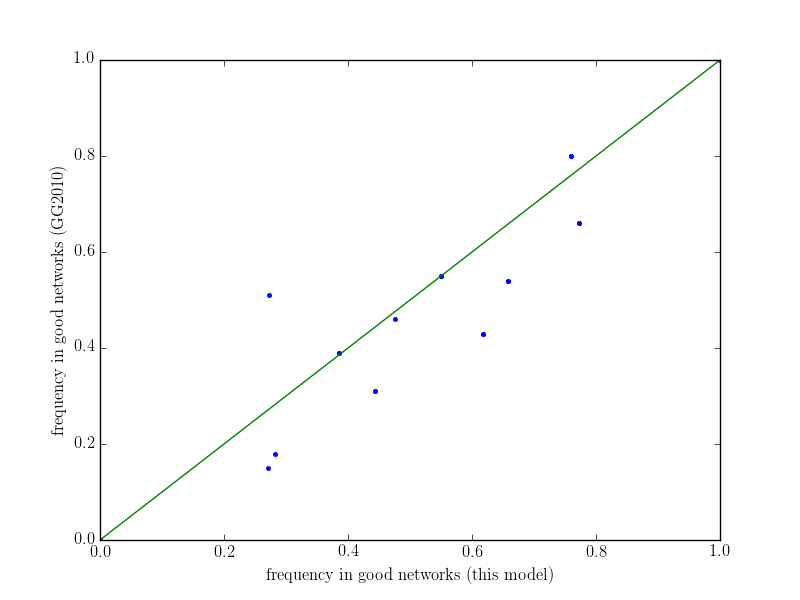
\includegraphics[width=0.7\textwidth,clip=true,trim=0cm 0cm 0cm 0cm]{freq-correlation.png}
    \label{fig:freq-correlation}}

\subfloat[]{
    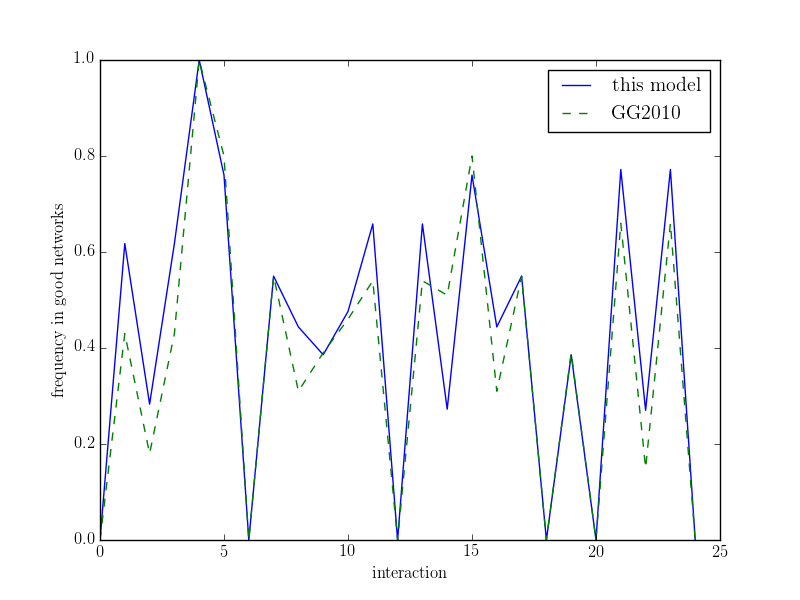
\includegraphics[width=0.7\textwidth,clip=true,trim=0cm 0cm 0cm 0cm]{freq-dist.png}
    \label{fig:freq-dist}}
  \caption{\emph{Frequency of interactions within successful networks}.\textbf{(a)} orders the interactions by how frequent they are in successful networks in the original model (GG2010). The interaction marked * is fixed in all networks and therefore must occur in 100\% of cases. The frequencies given by our model are remarkably similar. \textbf{(b)} plots the frequency of each interaction in both models with the line y = x showing a perfect correspondence. \textbf{(c)} has each x value as one of the 25 interactions, showing how close each models frequency distribution is.}
\end{figure}
\clearpage}

\subsection{The state space dynamics have some smoothness over networks}
An advantage of having a deterministic model is that it is possible to find the attractors for each network. We took all successful networks from our model and found their attractors (using the code in `bases.py'), which were then plotted in figure \ref{fig:attractors}. For comparison we also plotted the same number of random networks (figure \ref{fig:attractors-random}). Every network is ordered on the y-axis by its Hamming distance to a particular reference network. The clustering of similar dynamics indicates that there is some smoothness in the mapping from network-space to attractor-space, in other words networks that are close to each other are more similar than is typical. Another notable feature of figure \ref{fig:attractors-random} is that, even in random networks, point attractors (black dots) tend to be found at our desired locations (330 and 693) and rarely elsewhere. This suggests that our required states (opposing gradients) are special within the network space we are exploring, and will be due to the constraints set out in figure \ref{fig:table1}. 

\afterpage{
\begin{figure}
  \centering
\subfloat[]{
    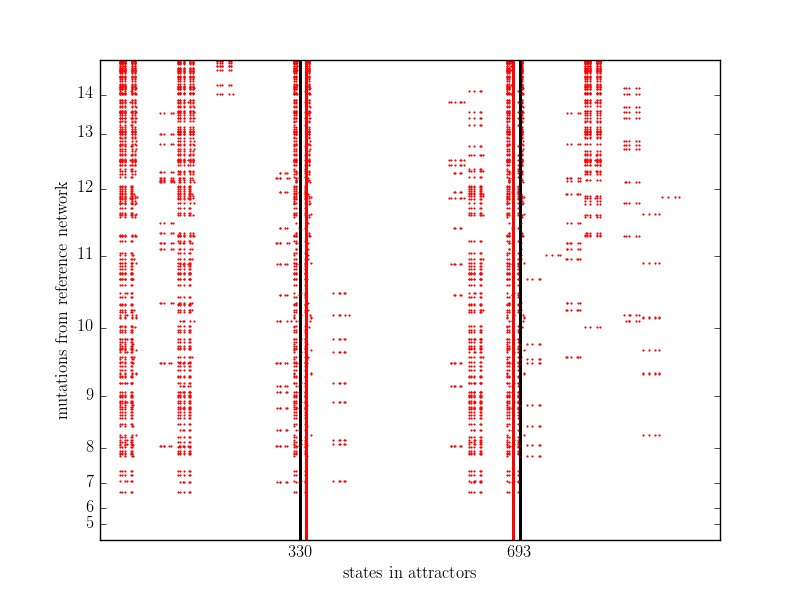
\includegraphics[width=0.7\textwidth,clip=true,trim=0cm 0cm 0cm 0cm]{attractors.png}
    \label{fig:attractors}}

\subfloat[]{
    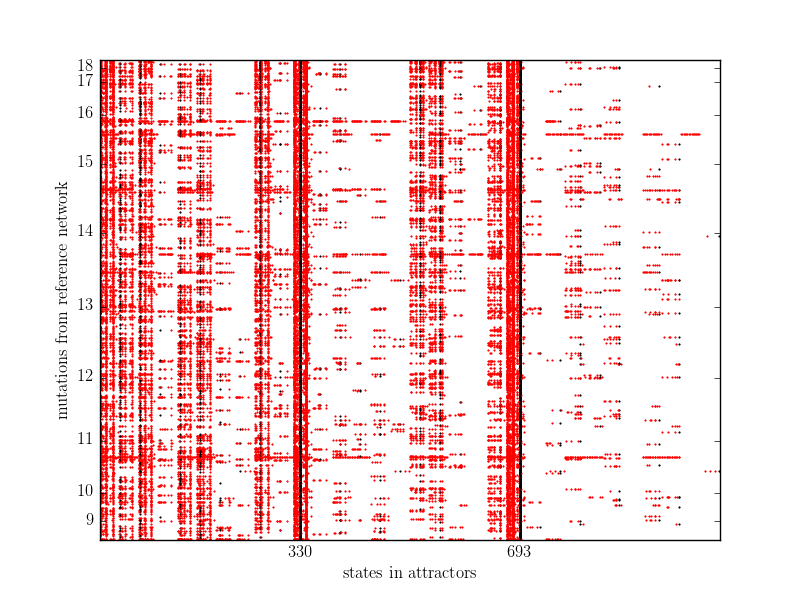
\includegraphics[width=0.7\textwidth,clip=true,trim=0cm 0cm 0cm 0cm]{attractors-random.png}
    \label{fig:attractors-random}}
  \caption{\emph{Attractor locations and type}.These figures plot the limit cycles and point attractors for \textbf{(a)} all successful networks and \textbf{(b)} the same number of random networks. The x-values are the limit-cycle states encoded as a decimal, the y-axis contains each network in order of its Hamming distance from a reference successful network. The black markers are point attractors, the red markers are states within limit-cycles. Some level of smoothness can be seen in figure \textbf{(a)} by the similarity of dynamics with distance from the reference network. The code to reproduce these plots is in `attractors.py'.}
\end{figure}
\clearpage}

\section{Results - Structure of fitness landscape}
\subsection{Comparison of null models}
The null models were designed to give landscapes which were perfectly rough or smooth, so that we can see what kind of statistics such landscapes will produce. The rough landscape was achieved by having a fitness function which simply returns a random number, in this way there is zero correlation between adjacent networks. In the evolutionary algorithm the parameter p determines how far away the next network tested will be. A value of p = 0.5 will pick the next network uniformly from across the entire network space, where as a small value like p = 0.1 will on average mutate $0.1\times80=8$ bits, selecting a network which is fairly close. As expected, in such a landscape the value of p in the evolutionary algorithm has no effect on the number of generations taken to reach the peak fitness (figure \ref{fig:rough}).\par

Compare this to a perfectly smooth landscape (figure \ref{fig:smooth}). In this case a decrease in the value of p also searches more proximate networks, however now the fitness of these networks is correlated, meaning fewer generations are required to find the peak. To understand why this is, consider a situation where we have selected a network with quite good fitness, say 0.7. At this point there are many more networks with lower fitness than there are with higher fitness, so selecting the next network from the entire space (p = 0.5) will rarely give us a fitter network. However, as p decreases so does the number of bits mutated, the range from which the next network is selected is brought closer in. As p approaches zero the proportion of networks which are fitter approaches 50\%, but only if the landscape is smooth.\par

\afterpage{
\begin{figure}
\centering
\subfloat[]{
    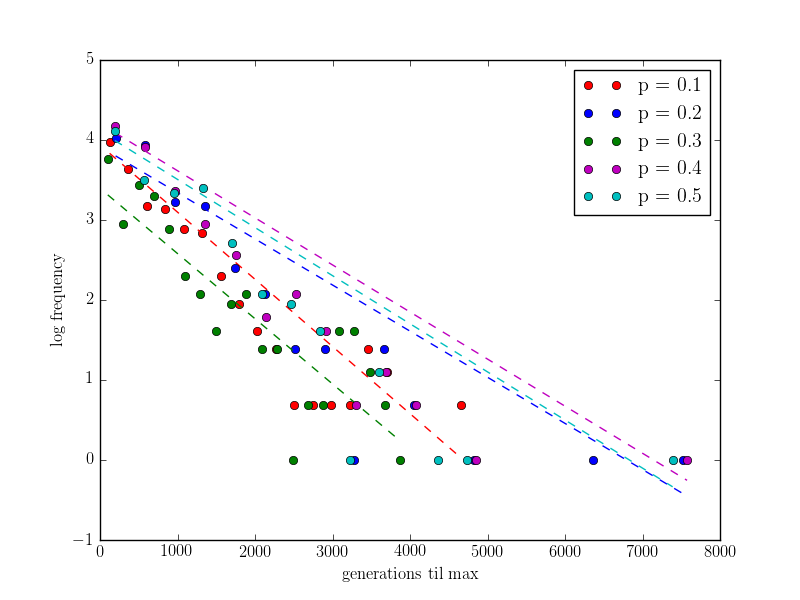
\includegraphics[width=0.7\textwidth,clip=true,trim=0cm 0cm 0cm 0cm]{rough.png}
    \label{fig:rough}}

 \subfloat[]{
    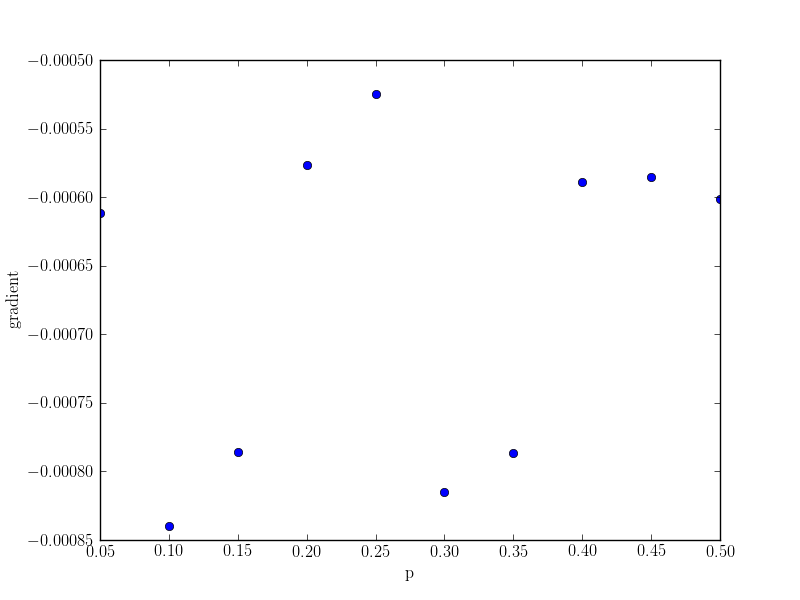
\includegraphics[width=0.7\textwidth,clip=true,trim=0cm 0cm 0cm 0cm]{roughslopes.png}
    \label{fig:roughslopes}}
  \caption{\emph{Distribution of generations taken to find maximum fitness - rough landscape}. Each generation the genome's fitness is measured, in this case it is a random number. Each bit in the genome is flipped with probability p. One trial consists of as many generations needed until the fitness has increased to its maximum. \textbf{(a)} shows the frequency of different trial lengths, in this rough landscape the value of p is irrelevant. \textbf{(b)} shows the gradients from \textbf{(a)}, a steeper gradient would mean the peak fitness is found faster, but in this case there is no correlation between p and rate of finding the peak. The code to reproduce these figures can be found in 'evolve.py'.}
\end{figure}
\clearpage}

\afterpage{
\begin{figure}
  \centering
\subfloat[]{
    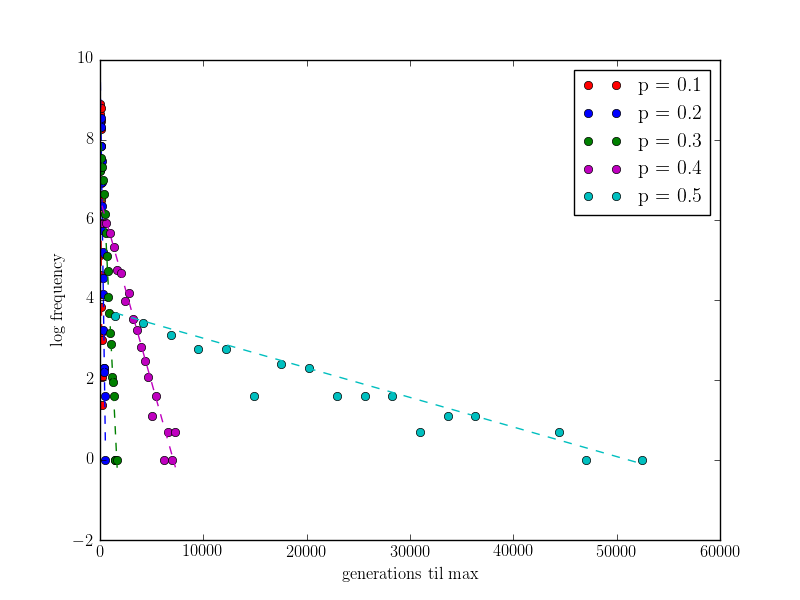
\includegraphics[width=0.7\textwidth,clip=true,trim=0cm 0cm 0cm 0cm]{smooth.png}
    \label{fig:smooth}}

\subfloat[]{
    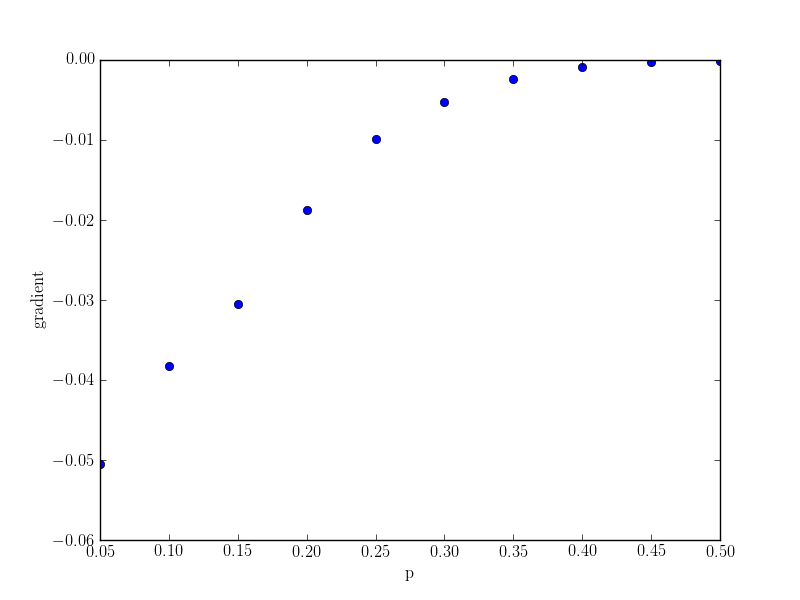
\includegraphics[width=0.7\textwidth,clip=true,trim=0cm 0cm 0cm 0cm]{smoothslopes.png}
    \label{fig:smoothslopes}}
  \caption{\emph{Distribution of generations taken to find maximum fitness - smooth landscape}. \textbf{(a)} In a perfectly smooth landscape the algorithm finds the peak much faster for smaller values of p. In this case lower p values have steeper gradients \textbf{(b)}, as they use the smoothness to approach the peak fitness faster. The code to reproduce these figures can be found in 'evolve.py'.}
\end{figure}
\clearpage}

\subsection{Our fitness function gives smooth landscape}

The fitness function which we chose as to be feasible in the context of cortical arealisation gives statistics similar to the smooth null model.\par

The fitness function is what maps the genotype space to the phenotype space, ideally we would like to visualise the fitness of the phenotypes as a landscape in a 2 or 3 dimensional plot. Unfortunately, our genotype space is 80 dimensional and so our method of visualisation is to get an evolutionary algorithm to explore the space.\par

The results of the evolutionary exploration show that the landscape has a degree of smoothness, with decreasing p values giving improved approaches to peak fitness (figure \ref{fig:f1}).\par

A second approach that we took to visualise this was to sample the networks surrounding a peak at various mutational distances away. Figure \ref{fig:peak} plots the proportion of non-zero fitness networks as a function of the distance away from the peak, for twenty peaks. In every case it can be seen that there is some smoothness leading up to each peak, with it becoming increasingly likely to find a fit network the closer you are to the peak.\par

However, just because our fitness function creates a landscape which is smooth does not mean that there is one large peak, as is the case in the smooth null model. It is possible that there are many peaks scattered throughout the genotype space. Out of the 80 bits in the genotype there are 10 which must remain fixed for every maximally fit network. These 10 bits encode that state `10101' and `01010' must lead to themselves, as point attractors. This leaves a further 70 bits completely free as we could find no further motifs within all the successful genomes.\par

\afterpage{
\begin{figure}
  \centering
\subfloat[]{
    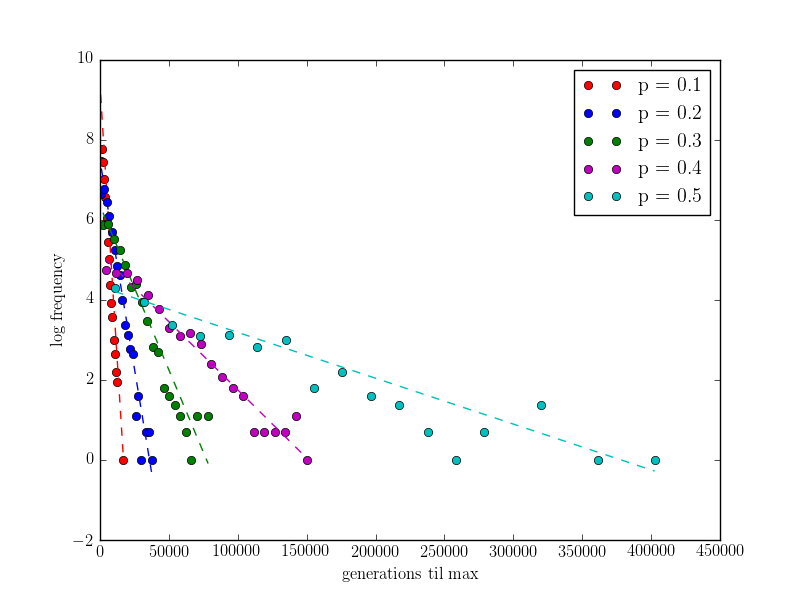
\includegraphics[width=0.8\textwidth,clip=true,trim=0cm 0cm 0cm 0cm]{f1.png}
    \label{fig:f1}}

\subfloat[]{
    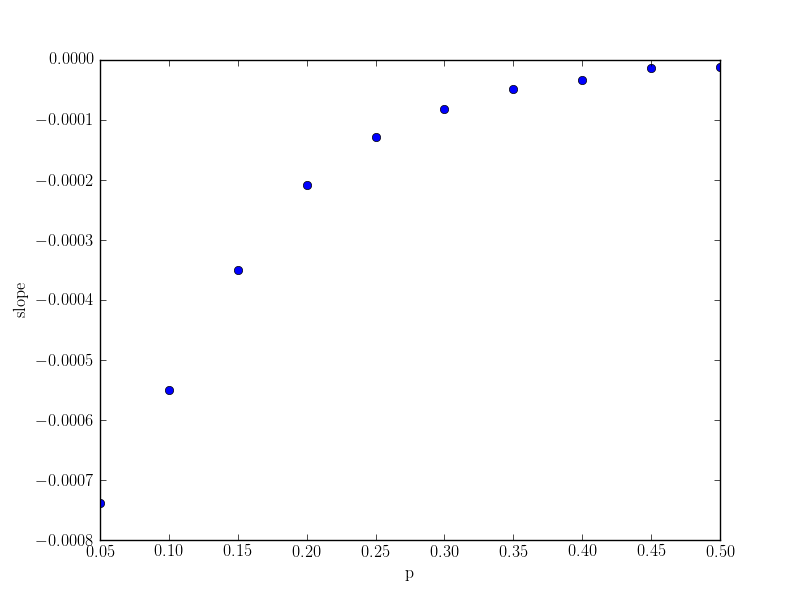
\includegraphics[width=0.8\textwidth,clip=true,trim=0cm 0cm 0cm 0cm]{f1slopes.png}
    \label{fig:f1slopes}}
  \caption{\emph{Distribution of generations taken to find maximum fitness - for our fitness landscape}. Our fitness function gives results similar to the smooth null model shown in figure \ref{fig:smooth}. The code to reproduce these figures can be found in 'evolve.py'.}
\end{figure}
\clearpage}


\afterpage{
\begin{figure}
\begin{center}
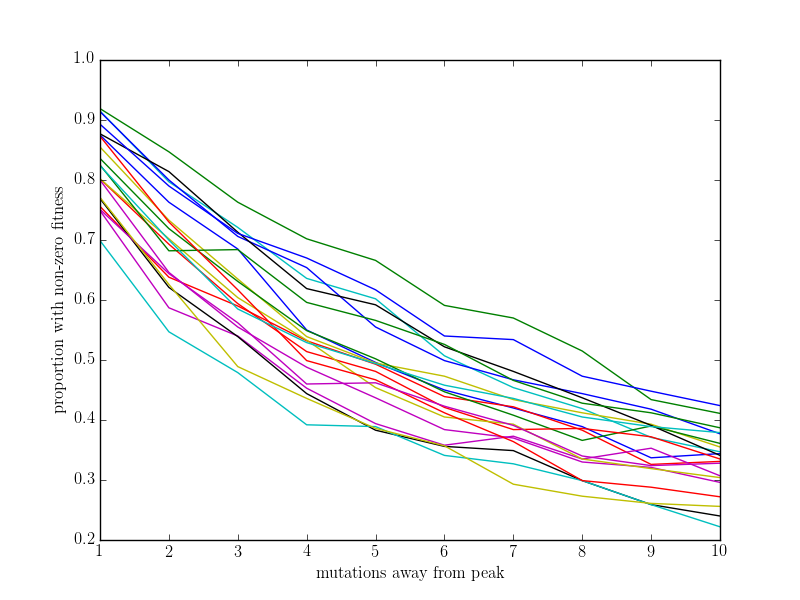
\includegraphics[width=1.0\textwidth,clip=true,trim=0cm 0cm 0cm 0cm]{peak.png}
  \caption{\emph{Values of fitness surrounding peaks}.Another indication of the smoothness in our landscape is found by counting how many surrounding networks have non-zero fitness. As we look further from the peak the proportion decreases exponentially. The code to reproduce this figure is in 'peak.py'}
  \label{fig:peak}
\end{center}
\end{figure}
\clearpage}


\subsection{Evolutionary search is up to 39 times faster than undirected search}

For each value of p we ran the evolutionary algorithm for 20,000,000 generations, the proportion of these generations which found the maximally fit state is shown in the table below. A p value of 0.5 is akin to searching the entire space uniformly randomly, as the value of each bit is independent of what it was before.\par
\vspace{2em}
\begin{center}
  \begin{tabular}{| r | r | l |} 
    \hline
    p & rate of finding optimal networks & rate relative to undirected search\\ 
    \hline  
    0.05 & 0.00055 & 39\\
    0.1 & 0.00044 & 31\\
    0.2 & 0.00019 & 14 \\
    0.3 & 0.000078 & 5.6 \\
    0.4 & 0.000035 & 2.5\\
    0.5 & 0.000014 & 1\\
    \hline
  \end{tabular}
\end{center}
\vspace{2em}

\newpage{}
\section{Discussion}
\subsection{A deterministic boolean network for cortical arealisation}
Boolean Networks are computationally simple models which have the potential to massively reduce the search space for feasible gene regulatory networks. However, there is also an enormous range of possible network parameters and assumptions, of which synchronocity is just one. To be reliable, the results of the model should be robust to small changes in these assumptions, or else there should be a strong biological explanation for why a particular set of assumptions is chosen.
\par

Although the best two networks from the Goodhill model were unsuccessful with this model (figs \ref{fig:best-a} and \ref{fig:best-b}), the similarity of the frequency distributions (figure \ref{fig:freq-dist}) suggests that the sets of successful networks are generally alike. However, a dose of mathematical caution is needed when interpreting the similarity of the frequency distributions. It is entirely possible that two completely different sets of networks have the same frequencies of interactions. In this case we are helped by the fact that both the original set of 5,849 good networks and our 1,710 successess are subsets of another set of 6,980, forcing them to have a conjunction. In Goodhill it was found that certain features such as inductive or repressive loops (eg. Fgf8 inhibits Emx2 which subsequently inhibits Fgf8) were never found in successful networks. Other failing features included autoregulation or the presence of nodes without regulators. Removing any networks with these features leaves a set of 6,980 networks which share the same frequency distribution as the successful networks. This means that the frequencies of interactions don't tell us anything special about the successful networks, except that they are part of the subset of networks not containing failing features. We therefore conclude that the situation is similar to that depicted in figure \ref{fig:venn}, and that there is a significant conjunction between the sets of successful networks from each model. 
\par

\afterpage{
\begin{figure}[h]
  \centering
  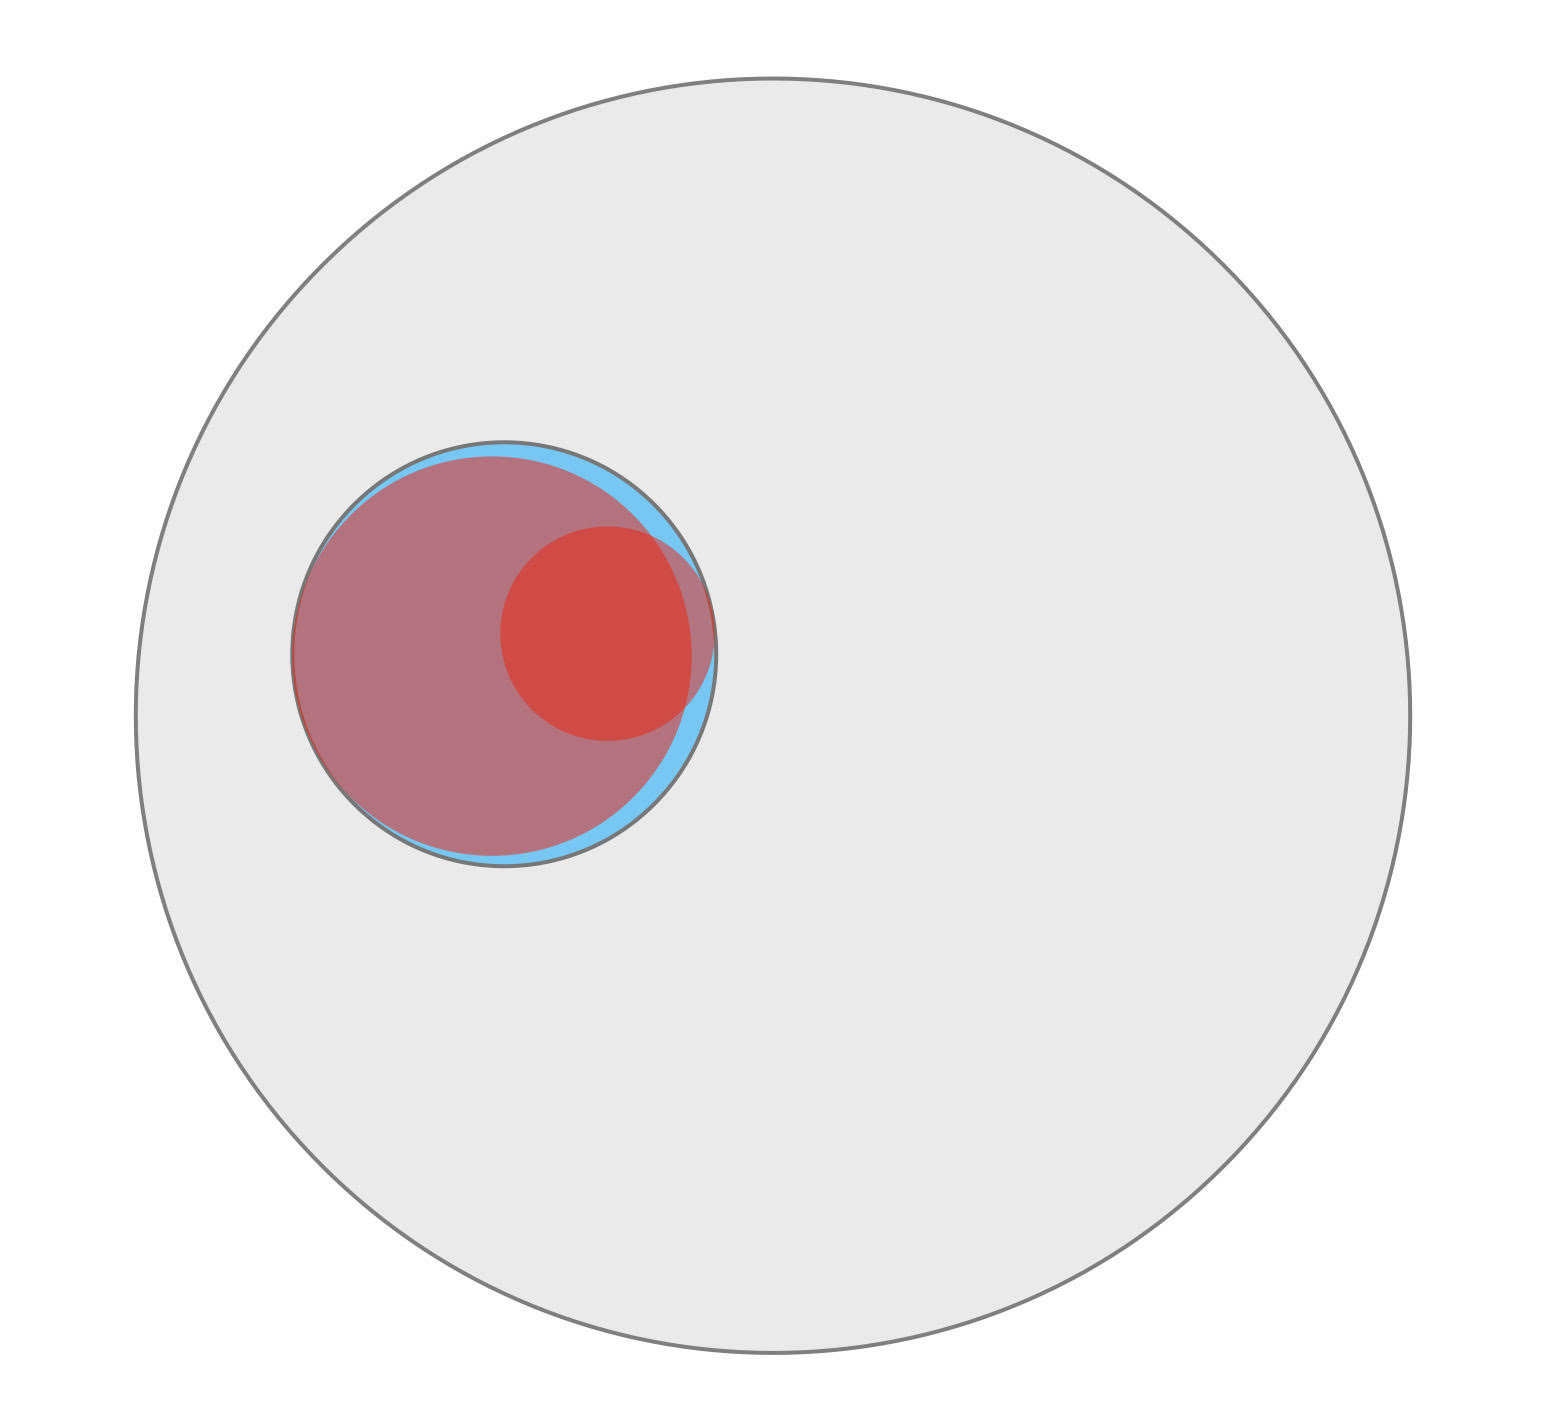
\includegraphics[width=1\textwidth,clip=true,trim=0cm 0cm 0cm 0cm]{venn.jpg}
  \caption{\emph{Conjunction of successful sets between models}. A venn diagram showing that there must be some conjunction between sets of successful networks from the two models (at least 579 networks but likely higher). The size of the largest circle is not to scale but the smaller circles' areas represent the number of networks in them. From largest to smallest the number of networks is $2^{24}, 6980, 5849, 1710$.}
  \label{fig:venn}
\end{figure}
\clearpage}

Unfortunately, without knowing the full set of networks which Goodhill found to be successful there is no way to tell which networks are successful in both models. We would like to obtain this data and do this simple comparison, which would also confirm the size of the conjunction.
\par

It seems that the results of the model are fairly invariant to the assumption of synchronicity, except that our synchronous model gave roughly three times fewer successful networks. This was extremely surprising given the debate around whether synchronous or asynchronous models are more appropriate. It suggests that either the asynchronicty in real biological networks is not an important detail, or that it is important but is not being accurately implemented in the models.
\par 

The opposing arguments in the debate are that synchronous models do not have realistic assumptions, or that asynchronous models do not give realistic dynamics. However both sides agree that asynchronicity completely alters the network dynamics \citep{Harvey1997}, where as we have found that an important result such as the frequency of interactions has actually remained the same.
\par

It is common in asynchronous models for most states to develop rapidly into a stable point attractor, rather than the interesting and diverse dynamics that are observed in real systems. Hallinan et al's solution is to expand the dichotomy of synchronous vs asynchronous into a continuous scale, meaning that each node is updated with probability p, where p = 1 would be a synchronous model \citep{Hallinan2004}. They find that `nearly' synchronous models (p = 0.9) give the most interesting dynamics. We think this is the reason our set of successful networks is three times smaller, there will be more states that drain into basins of attraction other than the desired stable points.
\par

Given that the models seem fairly robust, can we rely on them to produce accurate gene regulatory networks? There are some motifs that are common in real GRNs which are absent in our model. One of these is autoregulation, in all of our networks there are exactly zero self-inductive or self-inhibitory interactions, but this is a common feature of real biological systems \citep{Alon2007}. Another feature of real networks is that the number of inputs to any given node follows a power-law distribution, with more nodes with fewer inputs \citep{Koonin2011}. Taking the distribution for all of our networks shows this isn't the case for our model (figure \ref{fig:scaling}). However this may simply be because the networks are small, with only 1 to 4 interactions per node, and the relationship does seem to hold for 2-4 interactions.
\par

\afterpage{
\begin{figure}[h]
  \centering
  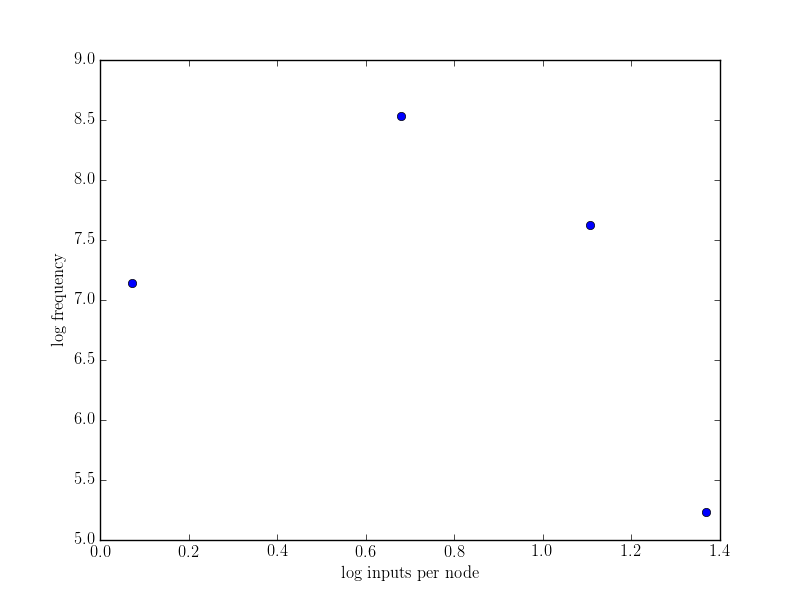
\includegraphics[width=1\textwidth,clip=true,trim=0cm 0cm 0cm 0cm]{scaling.png}
  \caption{\emph{Distribution of inputs per node}. It is common for real biological networks to have a decreasing power-law distribution for the number of interactions per node. This would give a straight line on this graph with a negative slope. The points plotted here are the frequency of inputs per node for all of our successful networks, where the power-law distribution does not hold, although there is a decrease in frequency for 2 to 4 interactions. The code in `scaling.py' will reproduce this figure.}
  \label{fig:scaling}
\end{figure}
\clearpage}

Another questionable aspect of our model networks is the degree to which the entire state space is important, or just the trajectory starting from a particular initial condition. In practically all these networks we get point attractors at 330 and 693, and also oscillators between 341 and 682. The former is perfect for establishing coritcal areas but the latter would be disastrous, with the gradients flipping back and forth. If we can be certain that initially it is only Fgf8 that is expressed, and only in the anterior domain, then it is not a problem. However any small deviation from this does seem feasible, in which case other trajectories would have to be considered.
\par

\subsection{Development accelerating evolution}

It has been shown that learning can change the phenotypic space which natural selection acts on, thus speeding up evolution \citep{Hinton1987}. This phenomena is an example of the Baldwin effect, which can also refer to developmental processes other than learning. Hinton and Nowlan argued that evolution may sometimes be required to find a `needle in a haystack', where there is one optimal phenotype in a large phenotypic space. This would appear as a fitness landscape with one sharp peak. What is required is a broadening of the peak so that the evolutionary process is more likely to find it. Hinton and Nowlan showed using a simulation that the process of learning can broaden that peak. In this thesis we have shown that the development of states in a Gene Regulatory Network can do the same.\par

It would be fair to argue that our model is too abstracted and not biologically plausible. For example, in organisms mutations are not applied to bits in truth tables. There is a complicated non-linear correspondence between the mutations in DNA and the logical functions of a regulatory network. Also, we have selected a fitness function that works for our purposes, but we do not know how incorrect gradients would really effect the fitness of an organism.\par

While biologically unrealistic, our model is designed to make a more general point about self-organisation, which is indeed prevalent in real biological systems. For a binary network of $N$ nodes there are $2^N$ possible states, however the network self-organises towards a smaller number of attractors. Sometimes a single mutation will radically alter the final states, as in figure \ref{fig:close}, but often the system will barely change. This robustness of the networks, combined with the fact that the genotypic space is highly dimensional and connected, means that there can be a correspondence between adjacent genomes and similar fitness values, in other words, smoothness. This is the case even when the genome seems completely uncorrelated with the phenome, as are our truth tables with the values of fitness.\par

It is common to explain biological features by how they have been selected for in an evolutionary process: the organism is this way because it has a successful adaptation. However, with epigenetics there are multiple evolutionary processes for the organism to be adapted with respect to. A genetic mutation could effect a phenotype directly, or via self-organisation in a regulatory network, or even by effecting the ability to learn. If one process allows the species fitness to increase more rapidly then it will be favoured. Almost like an evolutionary pressure on the method of adaptation itself. Finding which processes of mutation are more successful in different situations gives us another level by which to explain why an organism is the way it is.\par

\newpage{}
\bibliography{references}

\newpage{}
\section{Supporting Information}

\textbf{Source Code}. Source code to reproduce all figures can be found online at https://github.com/dan-whiteley/MScThesis

This is with the exception of figure \ref{fig:mammals}, which was copied from Krubitzer and Seelke, 2012.

\end{document}